\documentclass[12pt,a4paper]{report}

\usepackage[utf8]{inputenc}
\usepackage[T1]{fontenc}
\usepackage[french]{babel}
\usepackage{graphicx}
\usepackage{geometry}
\usepackage{lmodern}
\usepackage{fancyhdr}
\usepackage{titlesec}
\usepackage{tocloft}
\usepackage{hyperref}
\usepackage{float}
\usepackage{ragged2e}
\usepackage{booktabs}
\usepackage{array}
\usepackage{xcolor}
\usepackage{colortbl}
\usepackage{amsmath}
\usepackage{amssymb}
\usepackage{listings}
\usepackage{caption}
\usepackage{subcaption}
\usepackage{multirow}
\usepackage{enumitem}
\usepackage{mdframed}
\usepackage{tikz}

\hypersetup{colorlinks=true, linkcolor=black, urlcolor=blue, citecolor=black}
\geometry{margin=2.5cm}

% Couleurs personnalisees
\definecolor{bleu}{RGB}{26,83,122}
\definecolor{rouge}{RGB}{192,57,43}
\definecolor{vert}{RGB}{39,174,96}
\definecolor{orange}{RGB}{211,84,0}
\definecolor{grislight}{RGB}{245,245,245}
\definecolor{codebg}{RGB}{248,248,248}

% Style des titres de chapitres
\titleformat{\chapter}[display]
  {\normalfont\Large\bfseries\color{bleu}}
  {\chaptertitlename\ \thechapter}{12pt}{\Huge}

% Style des sections
\titleformat{\section}
  {\normalfont\large\bfseries\color{bleu}}
  {\thesection}{1em}{}

\titleformat{\subsection}
  {\normalfont\normalsize\bfseries\color{bleu!80!black}}
  {\thesubsection}{1em}{}

% Style du code Python
\lstdefinestyle{python}{
  language=Python,
  backgroundcolor=\color{codebg},
  basicstyle=\ttfamily\footnotesize,
  keywordstyle=\color{bleu}\bfseries,
  commentstyle=\color{gray},
  stringstyle=\color{rouge},
  frame=single,
  rulecolor=\color{bleu!30},
  breaklines=true,
  numbers=left,
  numberstyle=\tiny\color{gray},
  xleftmargin=15pt,
  captionpos=b
}

% En-tete et pied de page
\pagestyle{fancy}
\fancyhf{}
\fancyhead[L]{\small\textit{Pr\'{e}diction des feux de for\^{e}t par Deep Learning}}
\fancyhead[R]{\small\textit{EMSI Rabat --- 2025/2026}}
\fancyfoot[C]{\thepage}
\renewcommand{\headrulewidth}{0.4pt}

% Boite info
\newmdenv[
  linecolor=bleu,
  backgroundcolor=bleu!5,
  roundcorner=5pt,
  leftmargin=0, rightmargin=0,
  innerleftmargin=10pt, innerrightmargin=10pt,
  innertopmargin=8pt, innerbottommargin=8pt
]{infobox}

% ============================================================
\begin{document}

% ================= PAGE DE GARDE =================
\begin{titlepage}
\centering
\thispagestyle{empty}

\begin{minipage}{0.3\textwidth}
    \centering
    
\includegraphics[width=\textwidth]{img/ac3d23bf03508bcec887f3b9c26d414b562fda5f.png}
\end{minipage}
\hfill
\begin{minipage}{0.3\textwidth}
\centering
\end{minipage}
\hfill
\begin{minipage}{0.3\textwidth}
    \centering
    
\includegraphics[width=\textwidth]{img/fc3d0d2f2f510aaf50189e8c338b5c70872e730b.jpg}
\end{minipage}

\vspace{0.8cm}
{\Large \textbf{\'{E}cole Marocaine des Sciences de l'Ing\'{e}nieur --- Rabat}}\\[0.3cm]
{\large D\'{e}partement d'Informatique}\\[0.2cm]
{\large Fili\`{e}re : IA \& Data Science}

\vspace{1.2cm}
\rule{\textwidth}{1.5pt}\\[0.4cm]
{\Huge \textbf{Rapport de Projet Fin d'Ann\'{e}e}}\\[0.5cm]
{\LARGE \textcolor{bleu}{\textit{Pr\'{e}diction des feux de for\^{e}t bas\'{e}e\\[0.2cm] sur l'apprentissage profond}}}\\[0.3cm]
{\large Comparaison AlexNet-1D vs ResNet-1D sur donn\'{e}es MODIS --- Turquie 2020}\\[0.4cm]
\rule{\textwidth}{1.5pt}

\vspace{1.5cm}

\begin{minipage}{0.45\textwidth}
\textbf{R\'{e}alis\'{e} par :}
\begin{itemize}[noitemsep]
\item Yassine ERRAHMOUNI
\item Hafsa HOUSNI
\end{itemize}
\end{minipage}
\hfill
\begin{minipage}{0.45\textwidth}
\textbf{Encadr\'{e} par :}
\begin{itemize}[noitemsep]
\item Mme Aarich Mounia
\end{itemize}
\end{minipage}

\vfill
{\large Ann\'{e}e universitaire : 2025 --- 2026}
\end{titlepage}

% ================= REMERCIEMENTS =================
\chapter*{Remerciements}
\addcontentsline{toc}{chapter}{Remerciements}
\thispagestyle{fancy}

\justifying
Nous tenons \`{a} exprimer notre profonde gratitude \`{a} \textbf{Mme Aarich Mounia}, notre encadrante, pour son accompagnement bienveillant, ses conseils avis\'{e}s et sa disponibilit\'{e} tout au long de ce projet. Ses orientations nous ont permis d'approfondir nos connaissances en apprentissage profond et en data science appliqu\'{e}e.

Nous remercions \'{e}galement l'ensemble du corps enseignant du d\'{e}partement Informatique de l'\textbf{\'{E}cole Marocaine des Sciences de l'Ing\'{e}nieur de Rabat} pour la qualit\'{e} de la formation dispens\'{e}e et les solides bases th\'{e}oriques qu'ils nous ont transmises.

Nos remerciements vont aussi \`{a} \textbf{la NASA} pour la mise \`{a} disposition publique du syst\`{e}me \textbf{FIRMS (Fire Information for Resource Management System)} qui a fourni les donn\'{e}es MODIS utilis\'{e}es dans ce projet.

Enfin, nous remercions nos familles et nos proches pour leur soutien moral et leurs encouragements tout au long de cette ann\'{e}e universitaire.

% ================= RESUME =================
\chapter*{R\'{e}sum\'{e}}
\addcontentsline{toc}{chapter}{R\'{e}sum\'{e}}

\justifying
Ce projet de fin d'ann\'{e}es porte sur la classification automatique des types de feux de for\^{e}t \`{a} partir des donn\'{e}es satellitaires \textbf{MODIS} (Moderate Resolution Imaging Spectroradiometer) enregistr\'{e}es en \textbf{Turquie} durant l'ann\'{e}e \textbf{2020}. Le dataset contient 8~834 observations d\'{e}crites par 15 variables incluant des mesures thermiques (brightness, FRP), g\'{e}ographiques (latitude, longitude) et temporelles.

Face au fort d\'{e}s\'{e}quilibre des classes (92,9~\% de feux de v\'{e}g\'{e}tation contre 7~\% de volcans et 0,08~\% d'autres sources), deux strat\'{e}gies de r\'{e}\'{e}quilibrage sont compar\'{e}es : les \textbf{poids de classes} (\textit{class\_weight}) et le \textbf{sur-\'{e}chantillonnage synth\'{e}tique} (SMOTE). Deux architectures CNN~1D adapt\'{e}es aux donn\'{e}es tabulaires sont impl\'{e}ment\'{e}es sous Keras/TensorFlow : une inspir\'{e}e d'\textbf{AlexNet} et une inspir\'{e}e de \textbf{ResNet}.

Les r\'{e}sultats montrent que \textbf{ResNet-1D avec SMOTE} obtient les meilleures performances avec un F1-score pond\'{e}r\'{e} de \textbf{90,67~\%} et un RMSE de \textbf{0,6249}. Une \textbf{application web interactive} (\textit{FireRisk AI}) d\'{e}velopp\'{e}e avec Streamlit permet la pr\'{e}diction en temps r\'{e}el du risque d'incendie avec s\'{e}lection de localisation par carte interactive.

\vspace{0.5cm}
\noindent\textbf{Mots-cl\'{e}s :} Feux de for\^{e}t, MODIS, CNN 1D, AlexNet, ResNet, SMOTE, class\_weight, d\'{e}s\'{e}quilibre des classes, classification, deep learning, Streamlit.

% ================= ABSTRACT =================
\chapter*{Abstract}
\addcontentsline{toc}{chapter}{Abstract}

\justifying
This final-year project focuses on the automatic classification of wildfire types from \textbf{MODIS} satellite data recorded in \textbf{Turkey} during \textbf{2020}. The dataset contains 8,834 observations described by 15 variables including thermal measurements (brightness, FRP), geographic coordinates, and temporal features.

Given the severe class imbalance (92.9\% vegetation fires, 7\% volcanic activity, 0.08\% other sources), two rebalancing strategies are compared: \textbf{class weighting} and \textbf{SMOTE}. Two 1D CNN architectures adapted to tabular data are implemented: one inspired by \textbf{AlexNet} and one by \textbf{ResNet}. ResNet-1D with SMOTE achieves the best performance: weighted F1-score of \textbf{90.67\%} and RMSE of \textbf{0.6249}. An interactive web application (\textit{FireRisk AI}) provides real-time fire risk prediction with map-click-based location selection.

\vspace{0.5cm}
\noindent\textbf{Keywords:} Wildfire, MODIS, 1D CNN, AlexNet, ResNet, SMOTE, class imbalance, classification, deep learning, Streamlit.

% ================= LISTES =================
\listoffigures
\addcontentsline{toc}{chapter}{Liste des figures}

\listoftables
\addcontentsline{toc}{chapter}{Liste des tableaux}

\tableofcontents

% ================= INTRODUCTION GENERALE =================
\chapter*{Introduction g\'{e}n\'{e}rale}
\addcontentsline{toc}{chapter}{Introduction g\'{e}n\'{e}rale}

\justifying
Les feux de for\^{e}t repr\'{e}sentent aujourd'hui une menace majeure pour l'environnement, la biodiversit\'{e} et les populations humaines. Avec l'augmentation des temp\'{e}ratures mondiales li\'{e}e au changement climatique, la fr\'{e}quence et l'intensit\'{e} des incendies ne cessent de cro\^{i}tre. L'ann\'{e}e 2020 en Turquie a notamment connu une saison d'incendies particuli\`{e}rement d\'{e}vastatrice, avec des milliers d'hectares r\'{e}duits en cendres.

Gr\^{a}ce aux avanc\'{e}es r\'{e}centes en \textbf{apprentissage profond} (\textit{deep learning}), il est d\'{e}sormais possible d'analyser de grandes quantit\'{e}s de donn\'{e}es satellitaires afin d'identifier des patterns complexes et d'anticiper les risques d'incendie.

Ce projet vise \`{a} concevoir un \textbf{syst\`{e}me intelligent de classification des types de feux} bas\'{e} sur des architectures CNN~1D, et \`{a} le d\'{e}ployer sous forme d'application web interactive.

\medskip
\textbf{Organisation du rapport :}
\begin{itemize}
    \item \textbf{Chapitre 1} --- \'{E}tude th\'{e}orique : IA, Machine Learning, Deep Learning
    \item \textbf{Chapitre 2} --- Dataset et analyse exploratoire des donn\'{e}es MODIS
    \item \textbf{Chapitre 3} --- Pr\'{e}traitement et gestion du d\'{e}s\'{e}quilibre des classes
    \item \textbf{Chapitre 4} --- Architectures CNN 1D : AlexNet-1D et ResNet-1D
    \item \textbf{Chapitre 5} --- R\'{e}sultats, \'{e}valuation et comparaison
    \item \textbf{Chapitre 6} --- Application web FireRisk AI
\end{itemize}

% ============================================================
% CHAPITRE 1 — ETUDE THEORIQUE
% ============================================================
\chapter{\'{E}tude th\'{e}orique}

\section{Introduction}

Dans ce chapitre, nous pr\'{e}sentons les concepts fondamentaux n\'{e}cessaires \`{a} la compr\'{e}hension de notre projet : intelligence artificielle, machine learning, deep learning, et les principales architectures CNN et RNN.

\section{Intelligence Artificielle}

L'intelligence artificielle (IA) est un domaine de l'informatique qui vise \`{a} concevoir des syst\`{e}mes capables de simuler l'intelligence humaine : apprendre, raisonner, percevoir et d\'{e}cider.

\begin{figure}[H]
    \centering
    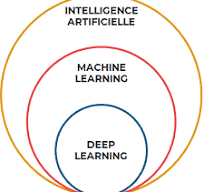
\includegraphics[width=0.65\textwidth]{img/Ia.png}
    \caption{Relation entre Intelligence Artificielle, Machine Learning et Deep Learning}
    \label{fig:ia}
\end{figure}

\section{Machine Learning}

Le machine learning est une sous-discipline de l'IA qui permet aux machines d'apprendre \`{a} partir de donn\'{e}es sans \^{e}tre explicitement programm\'{e}es.

\begin{figure}[H]
    \centering
    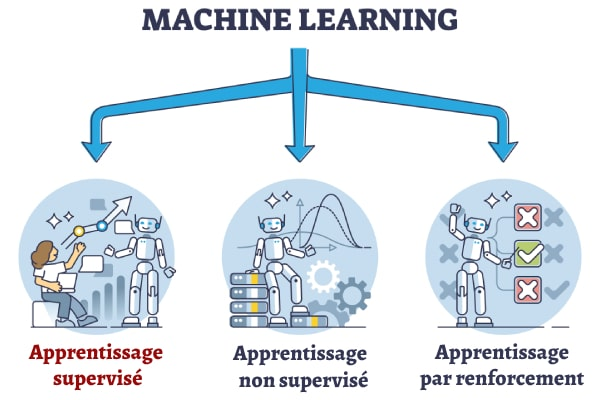
\includegraphics[width=0.7\textwidth]{img/ml_types.jpg}
    \caption{Les diff\'{e}rents types de Machine Learning}
    \label{fig:ml_types}
\end{figure}

\begin{table}[H]
\centering
\begin{tabular}{|>{\bfseries}p{3.5cm}|p{4.5cm}|p{4.5cm}|}
\hline
\rowcolor{bleu!15}
Type & Principe & Exemple \\
\hline
Supervis\'{e} & Donn\'{e}es \'{e}tiquet\'{e}es & Classification d'incendies \\
\hline
Non supervis\'{e} & D\'{e}tection de structures & Clustering de zones \`{a} risque \\
\hline
Par renforcement & R\'{e}compenses/p\'{e}nalit\'{e}s & Drones de surveillance \\
\hline
\end{tabular}
\caption{Comparaison des types d'apprentissage automatique}
\label{tab:ml_types}
\end{table}

Dans notre projet, nous utilisons l'\textbf{apprentissage supervis\'{e}} : chaque observation MODIS est associ\'{e}e \`{a} un label de type de feu (0, 2 ou 3).

\section{Deep Learning}

Le deep learning est bas\'{e} sur des r\'{e}seaux de neurones artificiels compos\'{e}s de plusieurs couches, capables de capturer des relations complexes dans les donn\'{e}es.

\subsection{R\'{e}seaux de neurones convolutifs (CNN)}

Les CNN exploitent la structure locale des donn\'{e}es via des filtres convolutifs. Originellement con\c{c}us pour les images, ils sont adaptables aux donn\'{e}es 1D (s\'{e}ries temporelles, donn\'{e}es tabulaires ordonn\'{e}es).

\begin{table}[H]
\centering
\begin{tabular}{|c|c|c|p{5cm}|}
\hline
\rowcolor{bleu!15}
\textbf{Architecture} & \textbf{Ann\'{e}e} & \textbf{Auteurs} & \textbf{Innovation principale} \\
\hline
LeNet & 1998 & Yann LeCun & Premier CNN convolutif \\
\hline
AlexNet & 2012 & Krizhevsky et al. & GPU + ReLU + Dropout \\
\hline
VGGNet & 2014 & Simonyan \& Zisserman & Filtres 3$\times$3, grande profondeur \\
\hline
ResNet & 2015 & Kaiming He & Connexions r\'{e}siduelles \\
\hline
Inception & 2014 & Google (Szegedy) & Multi-filtres en parall\`{e}le \\
\hline
DenseNet & 2017 & Huang et al. & Connexions denses \\
\hline
MobileNet & 2017 & Google & Convolutions s\'{e}parables \\
\hline
EfficientNet & 2019 & Tan \& Le & Mise \`{a} l'\'{e}chelle optimis\'{e}e \\
\hline
\end{tabular}
\caption{Principales architectures CNN et leurs innovations}
\label{tab:cnn_archi}
\end{table}

\subsubsection{LeNet (1998)}

\begin{figure}[H]
\centering
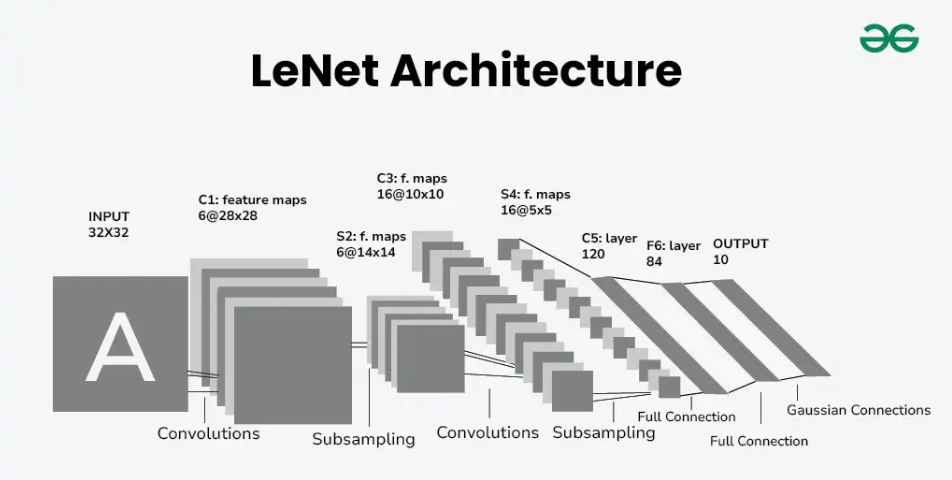
\includegraphics[width=0.75\textwidth]{img/Architecture LeNet.png}
\caption{Architecture LeNet --- premier r\'{e}seau convolutif}
\label{fig:lenet}
\end{figure}

LeNet, propos\'{e} par Yann LeCun, est le pr\'{e}curseur des CNN modernes. Compos\'{e} de blocs convolution-pooling suivis de couches denses, il a \'{e}t\'{e} con\c{c}u pour la reconnaissance de chiffres manuscrits (MNIST).

\subsubsection{AlexNet (2012)}

\begin{figure}[H]
\centering
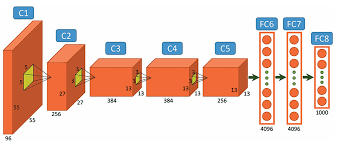
\includegraphics[width=0.8\textwidth]{img/alexNet.png}
\caption{Architecture AlexNet --- r\'{e}volution du deep learning}
\label{fig:alexnet}
\end{figure}

AlexNet a marqu\'{e} un tournant historique en remportant l'ILSVRC 2012. Il a introduit l'utilisation du GPU, la fonction d'activation ReLU et le Dropout. \textbf{Notre architecture AlexNet-1D s'inspire de cette philosophie} : blocs convolutifs s\'{e}quentiels + t\^{e}te de classification dense.

\subsubsection{VGGNet (2014)}

\begin{figure}[H]
\centering
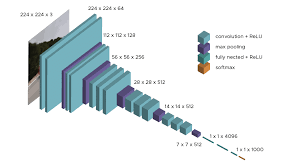
\includegraphics[width=0.75\textwidth]{img/vggnet.png}
\caption{Architecture VGGNet}
\label{fig:vgg}
\end{figure}

VGGNet a d\'{e}montr\'{e} qu'empiler de nombreux petits filtres (3$\times$3) est plus efficace que d'utiliser de grands filtres. Son architecture tr\`{e}s profonde reste une r\'{e}f\'{e}rence acad\'{e}mique.

\subsubsection{ResNet (2015)}

\begin{figure}[H]
\centering
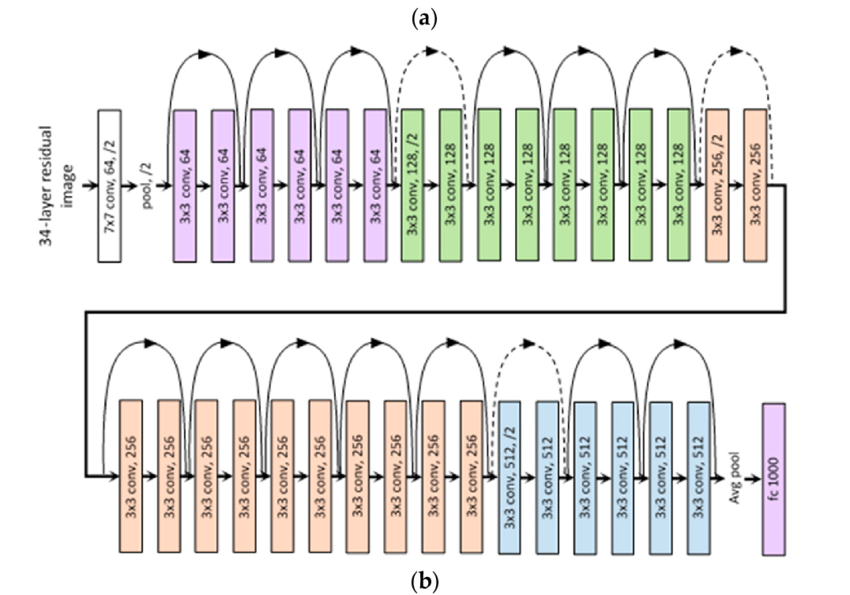
\includegraphics[width=0.8\textwidth]{img/Architecture ResNet.png}
\caption{Architecture ResNet et principe des connexions r\'{e}siduelles}
\label{fig:resnet_orig}
\end{figure}

ResNet a r\'{e}solu le probl\`{e}me du \textit{vanishing gradient} gr\^{a}ce aux \textbf{connexions r\'{e}siduelles} : $H(x) = F(x) + x$. Cette innovation permet d'entra\^{i}ner des r\'{e}seaux de plus de 100 couches. \textbf{Notre architecture ResNet-1D adapte ce principe aux donn\'{e}es tabulaires 1D.}

\subsubsection{Autres architectures CNN}

\begin{figure}[H]
\centering
\begin{subfigure}[b]{0.48\textwidth}
    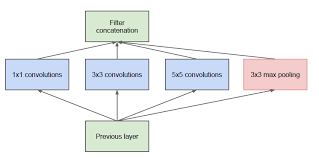
\includegraphics[width=\textwidth]{img/Architecture Inception.png}
    \caption{Architecture Inception (GoogleNet)}
\end{subfigure}
\hfill
\begin{subfigure}[b]{0.48\textwidth}
    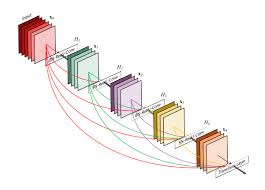
\includegraphics[width=\textwidth]{img/Architecture DenseNet.png}
    \caption{Architecture DenseNet}
\end{subfigure}
\caption{Architectures CNN avanc\'{e}es}
\label{fig:cnn_autres}
\end{figure}

\begin{figure}[H]
\centering
\begin{subfigure}[b]{0.48\textwidth}
    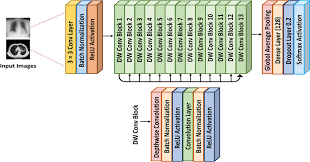
\includegraphics[width=\textwidth]{img/Architecture MobileNet.png}
    \caption{Architecture MobileNet}
\end{subfigure}
\hfill
\begin{subfigure}[b]{0.48\textwidth}
    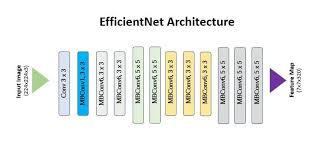
\includegraphics[width=\textwidth]{img/Architecture EfficientNet.png}
    \caption{Architecture EfficientNet}
\end{subfigure}
\caption{Architectures CNN l\'{e}g\`{e}res et efficaces}
\label{fig:cnn_light}
\end{figure}

\subsection{R\'{e}seaux de neurones r\'{e}currents (RNN)}

Les RNN sont adapt\'{e}s au traitement des donn\'{e}es s\'{e}quentielles. Ils maintiennent une m\'{e}moire interne permettant de capturer les d\'{e}pendances temporelles.

\begin{figure}[H]
\centering
\begin{subfigure}[b]{0.3\textwidth}
    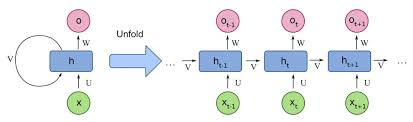
\includegraphics[width=\textwidth]{img/RNN classique.png}
    \caption{RNN classique}
\end{subfigure}
\hfill
\begin{subfigure}[b]{0.3\textwidth}
    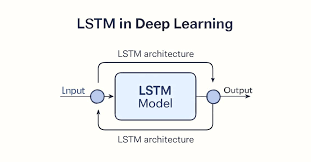
\includegraphics[width=\textwidth]{img/LSTM.png}
    \caption{LSTM}
\end{subfigure}
\hfill
\begin{subfigure}[b]{0.3\textwidth}
    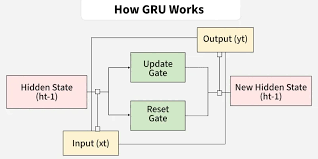
\includegraphics[width=\textwidth]{img/GRU.png}
    \caption{GRU}
\end{subfigure}
\caption{Architectures RNN : classique, LSTM et GRU}
\label{fig:rnn}
\end{figure}

\begin{table}[H]
\centering
\begin{tabular}{|c|c|p{6.5cm}|}
\hline
\rowcolor{bleu!15}
\textbf{Architecture} & \textbf{Ann\'{e}e} & \textbf{Avantage principal} \\
\hline
RNN classique & 1980s & Simple, m\'{e}moire court terme \\
\hline
LSTM & 1997 & M\'{e}moire long terme gr\^{a}ce aux portes \\
\hline
GRU & 2014 & Plus l\'{e}ger que LSTM, moins de param\`{e}tres \\
\hline
\end{tabular}
\caption{Comparaison des architectures RNN}
\label{tab:rnn}
\end{table}

\section{Conclusion}

Ce chapitre a pr\'{e}sent\'{e} les fondements th\'{e}oriques. Les architectures AlexNet et ResNet constituent les inspirations directes de nos mod\`{e}les CNN~1D d\'{e}velopp\'{e}s dans les chapitres suivants.

% ============================================================
% CHAPITRE 2 — DATASET ET EDA
% ============================================================
\chapter{Pr\'{e}sentation du Dataset et Analyse Exploratoire}

\section{Introduction}

Ce chapitre pr\'{e}sente le dataset MODIS utilis\'{e} et les observations issues de l'analyse exploratoire (EDA) qui ont guid\'{e} les choix de pr\'{e}traitement.

\section{Source des donn\'{e}es}

\begin{infobox}
\textbf{NASA FIRMS (Fire Information for Resource Management System)}\\
Satellite : MODIS (Terra et Aqua) \quad --- \quad P\'{e}riode : Ann\'{e}e 2020 \quad --- \quad R\'{e}gion : Turquie
\end{infobox}

Le syst\`{e}me FIRMS de la NASA diffuse en temps quasi-r\'{e}el les d\'{e}tections actives de feux. Deux capteurs assurent une couverture double quotidienne : \textbf{Terra (A)} le matin et \textbf{Aqua (B)} l'apr\`{e}s-midi.

\section{Caract\'{e}ristiques g\'{e}n\'{e}rales}

\begin{table}[H]
\centering
\begin{tabular}{|>{\bfseries}l|l|}
\hline
\rowcolor{bleu!10}
Propri\'{e}t\'{e} & Valeur \\
\hline
Dimensions & 8~834 lignes $\times$ 15 colonnes \\
\hline
Valeurs manquantes & Aucune (dataset complet) \\
\hline
Variable cible & \texttt{type} (0 = v\'{e}g\'{e}tation, 2 = volcan, 3 = autre) \\
\hline
P\'{e}riode & Janvier -- D\'{e}cembre 2020 \\
\hline
R\'{e}gion & Territoire turc (lat. 35\degr--42\degr N, lon. 25\degr--45\degr E) \\
\hline
\end{tabular}
\caption{Caract\'{e}ristiques g\'{e}n\'{e}rales du dataset MODIS Turquie 2020}
\label{tab:dataset_info}
\end{table}

\section{Description des colonnes}

\begin{table}[H]
\centering
\small
\begin{tabular}{|l|c|p{5cm}|c|}
\hline
\rowcolor{bleu!15}
\textbf{Colonne} & \textbf{Type} & \textbf{Description} & \textbf{Statut} \\
\hline
\texttt{latitude} & float & Latitude GPS du foyer (°N) & Feature \\
\hline
\texttt{longitude} & float & Longitude GPS du foyer (°E) & Feature \\
\hline
\texttt{brightness} & float & Temp. brillance canal 21/22 (K) & Feature \\
\hline
\texttt{scan} & float & Taille pixel -- sens balayage (km) & Feature \\
\hline
\texttt{track} & float & Taille pixel -- sens d\'{e}placement (km) & Feature \\
\hline
\texttt{acq\_date} & string & Date d'acquisition (YYYY-MM-DD) & $\rightarrow$ mois extrait \\
\hline
\texttt{acq\_time} & int & Heure d'acquisition (HHMM) & $\rightarrow$ heure extraite \\
\hline
\texttt{satellite} & string & 'A' (Terra) ou 'B' (Aqua) & Encod\'{e}e 0/1 \\
\hline
\texttt{instrument} & string & Toujours 'MODIS' -- constante & \textcolor{rouge}{Supprim\'{e}e} \\
\hline
\texttt{confidence} & int & Confiance MODIS (0--100) & Feature \\
\hline
\texttt{version} & float & Toujours 6.03 -- constante & \textcolor{rouge}{Supprim\'{e}e} \\
\hline
\texttt{bright\_t31} & float & Temp. brillance canal 31 (K) & Feature \\
\hline
\texttt{frp} & float & Fire Radiative Power (MW/sr/m\textsuperscript{2}) & Feature \\
\hline
\texttt{daynight} & string & 'D' (diurne) ou 'N' (nocturne) & Encod\'{e}e 0/1 \\
\hline
\texttt{type} & int & Type de feu -- \textbf{variable cible} & \textbf{CIBLE} \\
\hline
\end{tabular}
\caption{Description des 15 colonnes du dataset MODIS}
\label{tab:colonnes}
\end{table}

\section{D\'{e}s\'{e}quilibre des classes}

\begin{table}[H]
\centering
\begin{tabular}{|c|l|r|r|r|}
\hline
\rowcolor{bleu!15}
\textbf{Classe} & \textbf{Label} & \textbf{Effectif} & \textbf{Proportion} & \textbf{Ratio vs Classe 3} \\
\hline
\rowcolor{rouge!10}
0 & V\'{e}g\'{e}tation (Vegetation fire) & 8~208 & 92,9\% & 1~172 : 1 \\
\hline
\rowcolor{orange!10}
2 & Volcan / Activit\'{e} g\'{e}othermique & 619 & 7,0\% & 88 : 1 \\
\hline
\rowcolor{vert!10}
3 & Autre source statique & 7 & 0,08\% & 1 : 1 \\
\hline
\end{tabular}
\caption{Distribution de la variable cible -- d\'{e}s\'{e}quilibre extr\^{e}me}
\label{tab:classes}
\end{table}

\begin{infobox}
Un classifieur na\"{i}f pr\'{e}disant toujours la classe~0 atteindrait 92,9\% d'accuracy sans rien apprendre. C'est pourquoi le \textbf{F1-score pond\'{e}r\'{e}} est la m\'{e}trique principale.
\end{infobox}

\section{Analyse exploratoire}

\subsection{Distribution de la variable cible}

\begin{figure}[H]
    \centering
    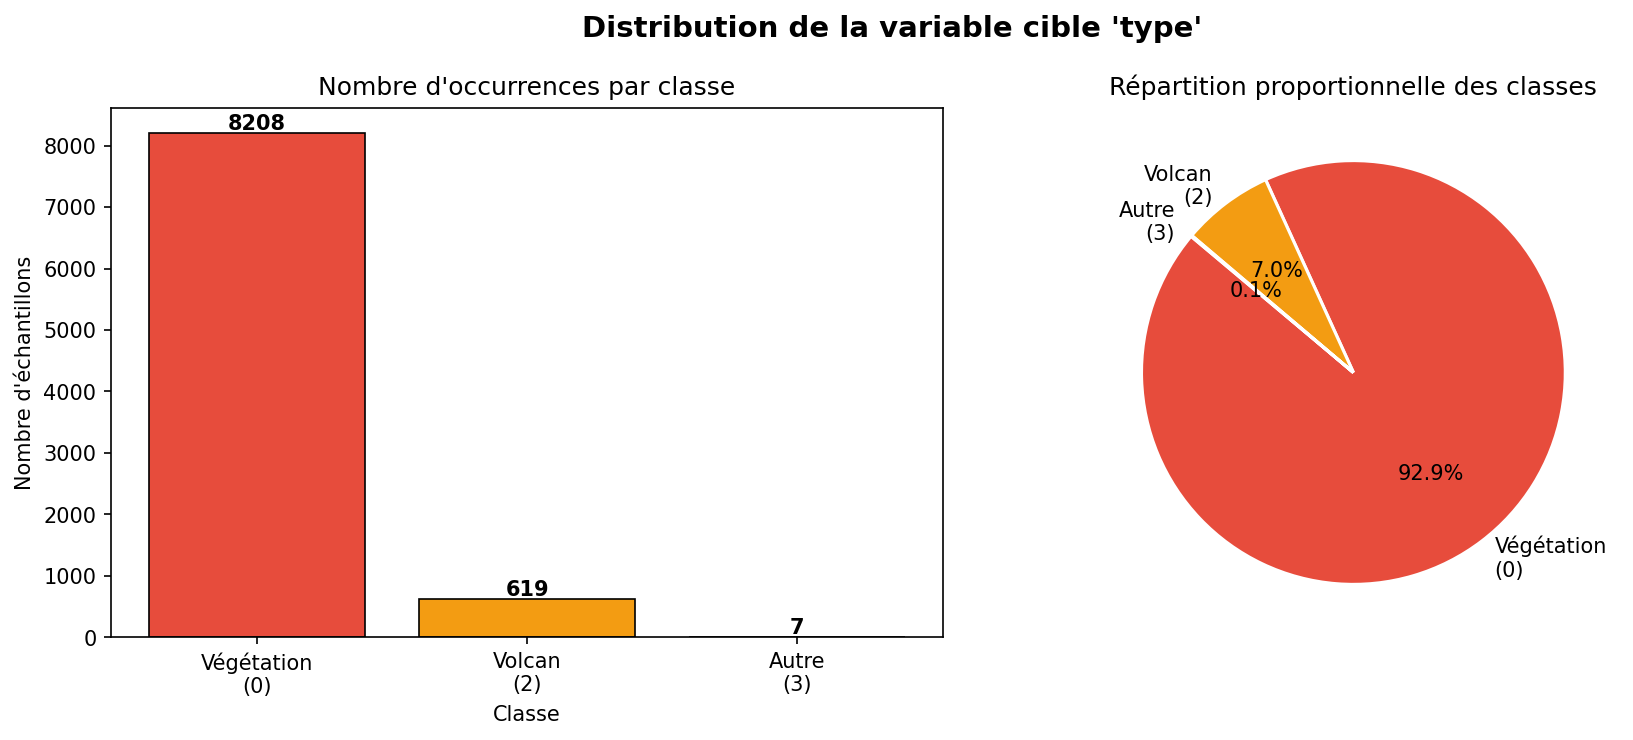
\includegraphics[width=\textwidth]{img/01_distribution_cible.png}
    \caption{Distribution de la variable cible 'type'}
    \label{fig:distrib_cible}
\end{figure}

\subsection{Distributions des features num\'{e}riques}

\begin{figure}[H]
    \centering
    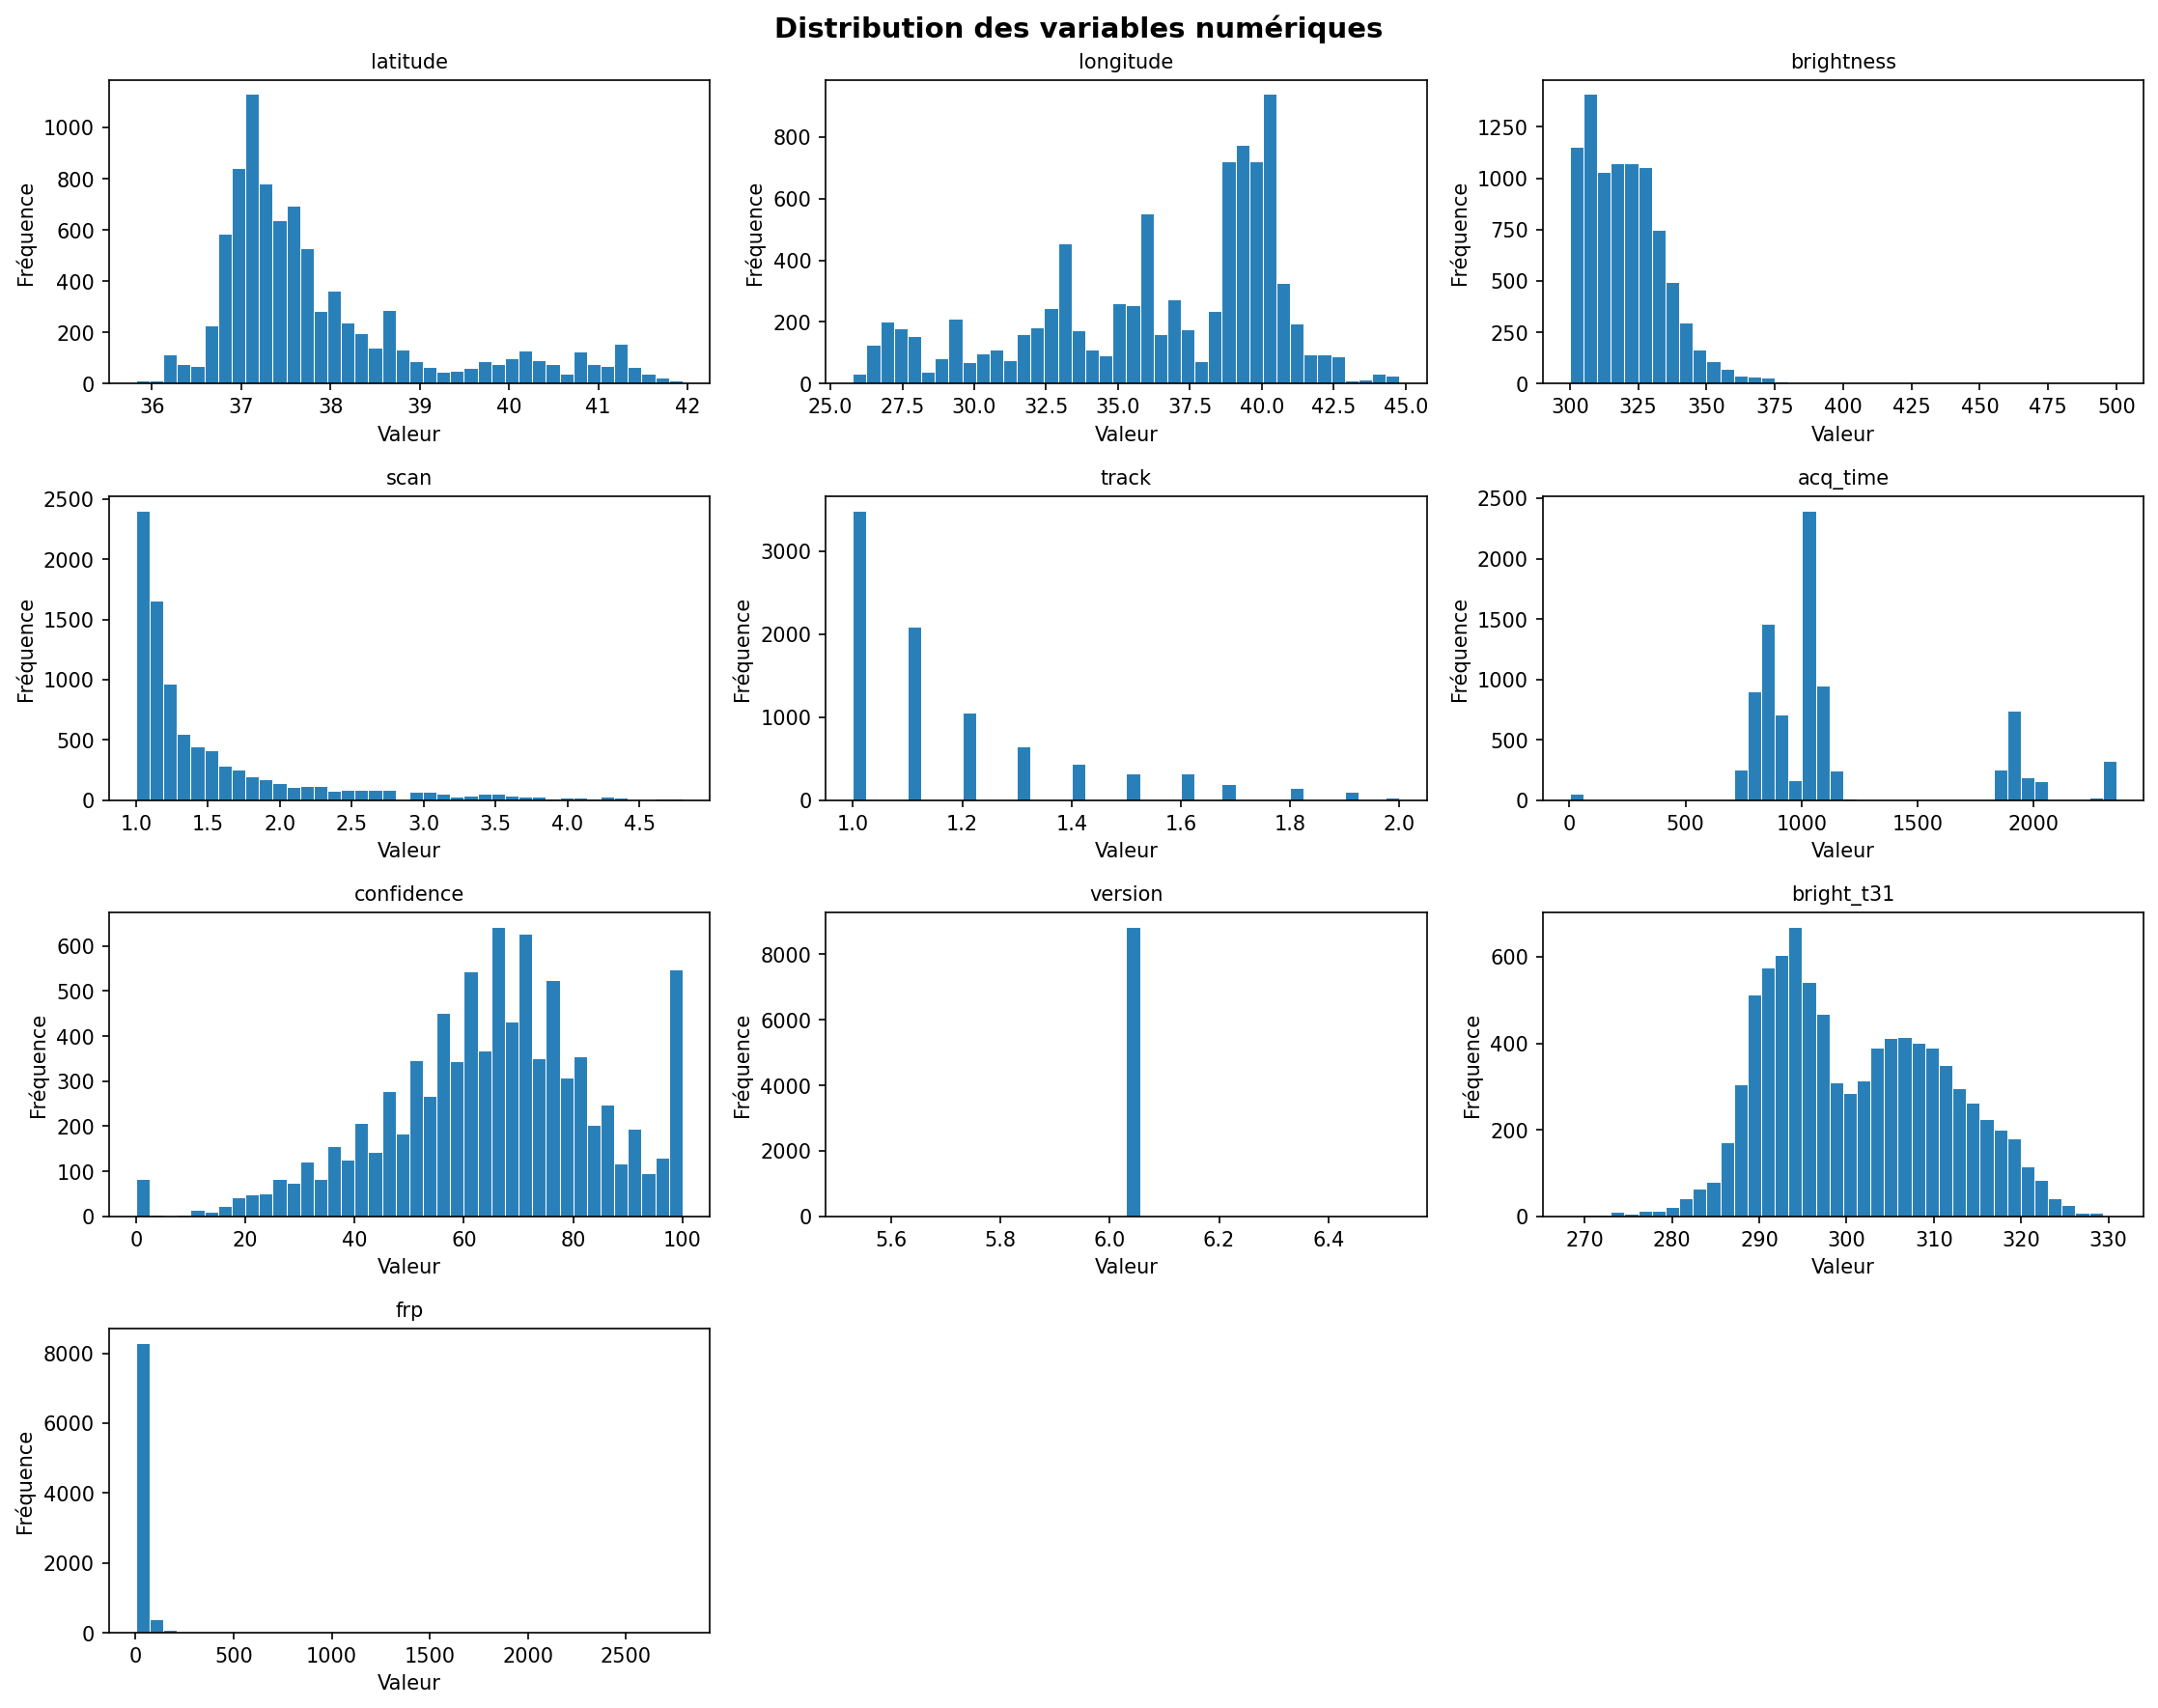
\includegraphics[width=\textwidth]{img/02_distributions_features.png}
    \caption{Histogrammes des variables num\'{e}riques}
    \label{fig:distrib_features}
\end{figure}

\begin{itemize}
    \item \textbf{brightness} : distribution quasi-normale centr\'{e}e \`{a} $\sim$320~K
    \item \textbf{frp} : tr\`{e}s asym\'{e}trique \`{a} droite, majorit\'{e} des valeurs $<$ 50~MW
    \item \textbf{confidence} : \'{e}tal\'{e} de 0 \`{a} 100\%, pic entre 60 et 80\%
\end{itemize}

\subsection{Matrice de corr\'{e}lation}

\begin{figure}[H]
    \centering
    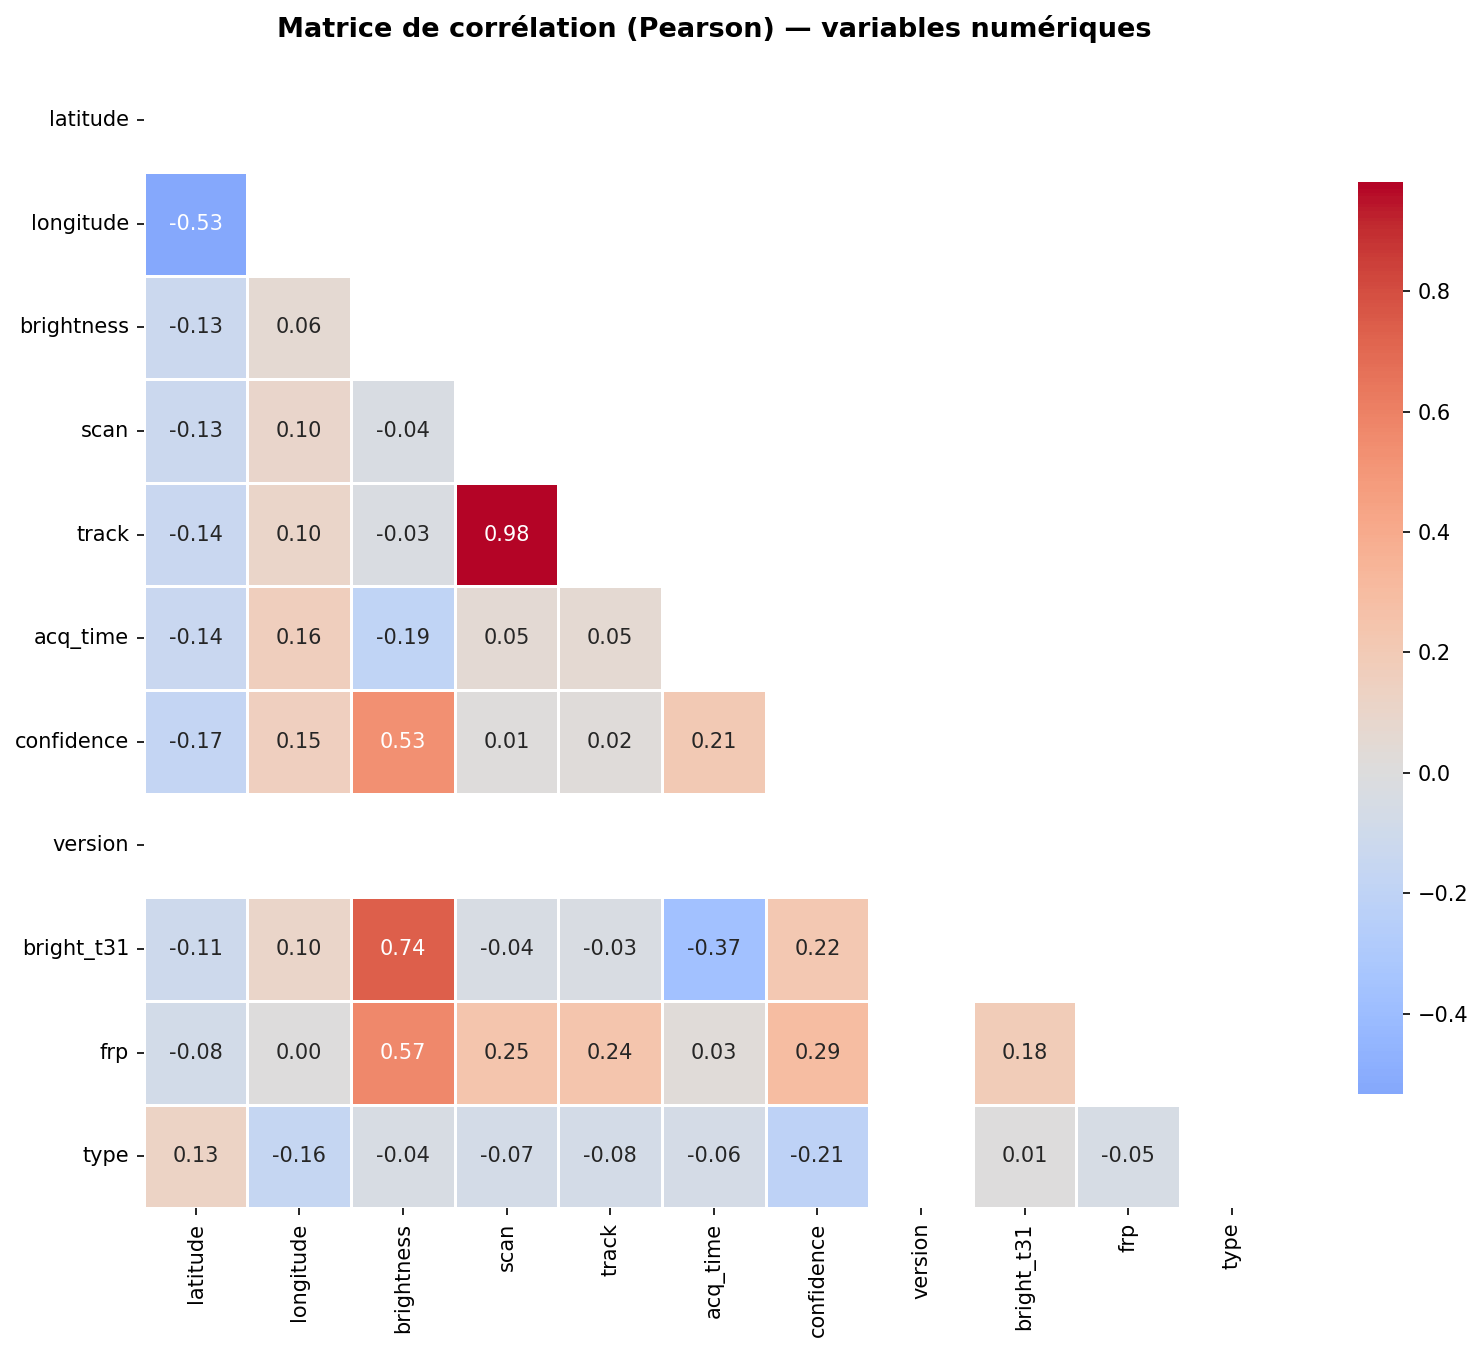
\includegraphics[width=0.9\textwidth]{img/03_matrice_correlation.png}
    \caption{Matrice de corr\'{e}lation de Pearson (triangle inf\'{e}rieur)}
    \label{fig:correlation}
\end{figure}

\begin{itemize}
    \item \textbf{brightness $\leftrightarrow$ bright\_t31} : corr\'{e}lation forte ($r > 0{,}7$) -- m\^{e}me ph\'{e}nom\`{e}ne physique
    \item \textbf{scan $\leftrightarrow$ track} : corr\'{e}lation forte -- g\'{e}om\'{e}trie satellite
    \item \textbf{frp} : feature la plus corr\'{e}l\'{e}e avec \texttt{type} -- meilleur pr\'{e}dicteur
\end{itemize}

\subsection{Boxplots par classe}

\begin{figure}[H]
    \centering
    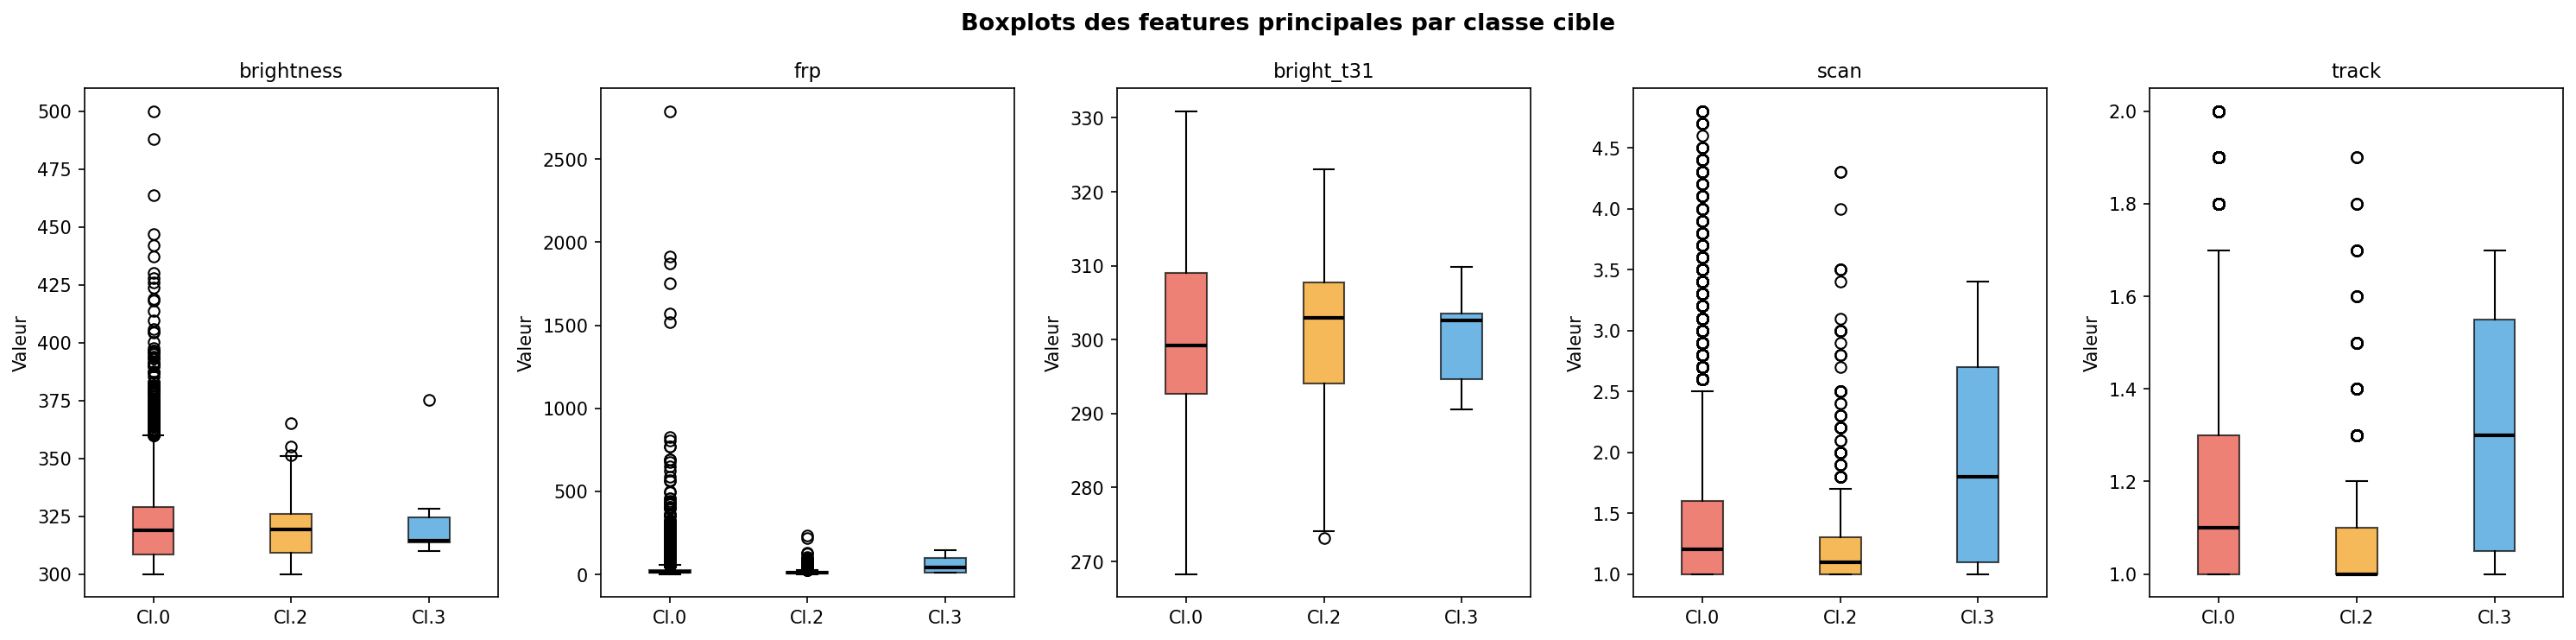
\includegraphics[width=\textwidth]{img/04_boxplots_par_classe.png}
    \caption{Boxplots des features principales selon le type de feu}
    \label{fig:boxplots}
\end{figure}

\subsection{Analyse temporelle}

\begin{figure}[H]
    \centering
    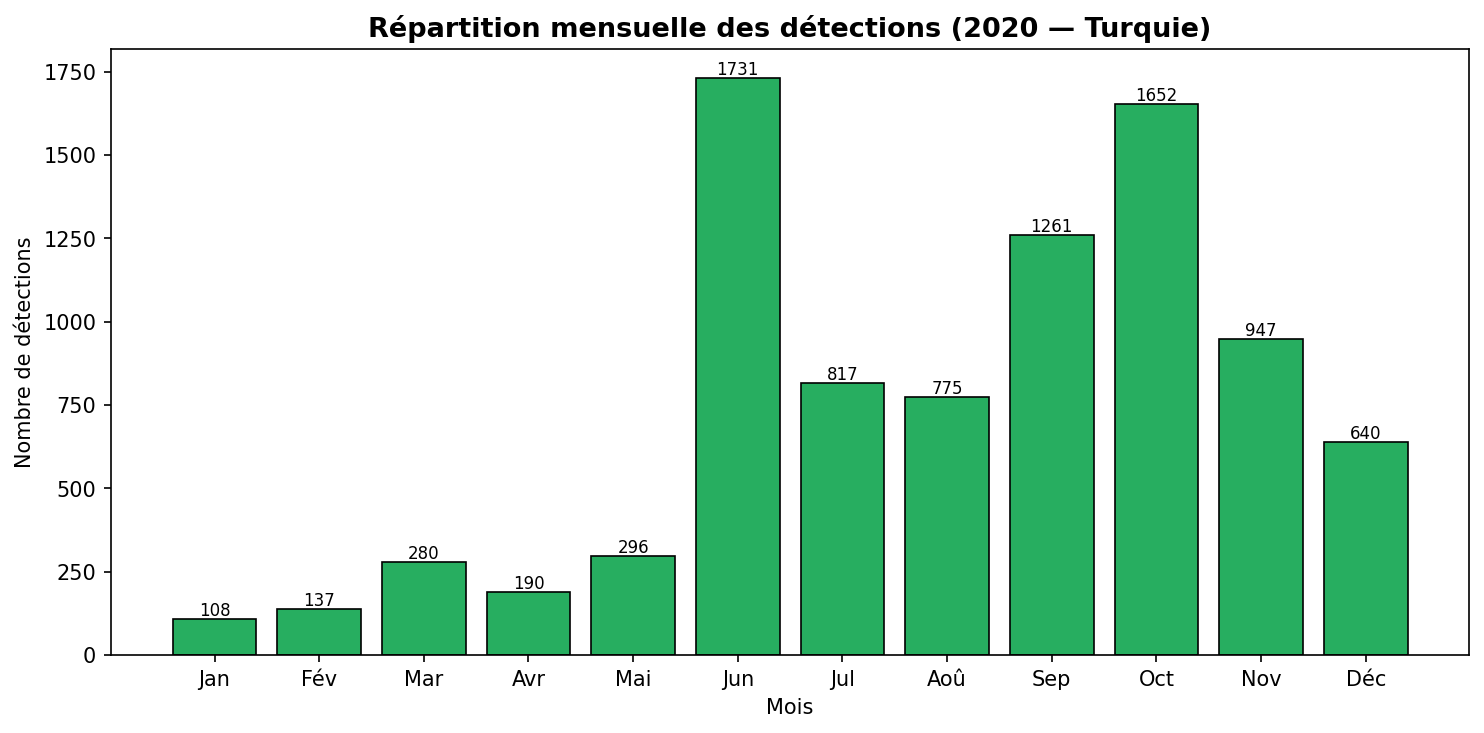
\includegraphics[width=\textwidth]{img/05_repartition_mensuelle.png}
    \caption{R\'{e}partition mensuelle -- pic estival juillet--septembre}
    \label{fig:mensuel}
\end{figure}

\subsection{R\'{e}partition g\'{e}ographique}

\begin{figure}[H]
    \centering
    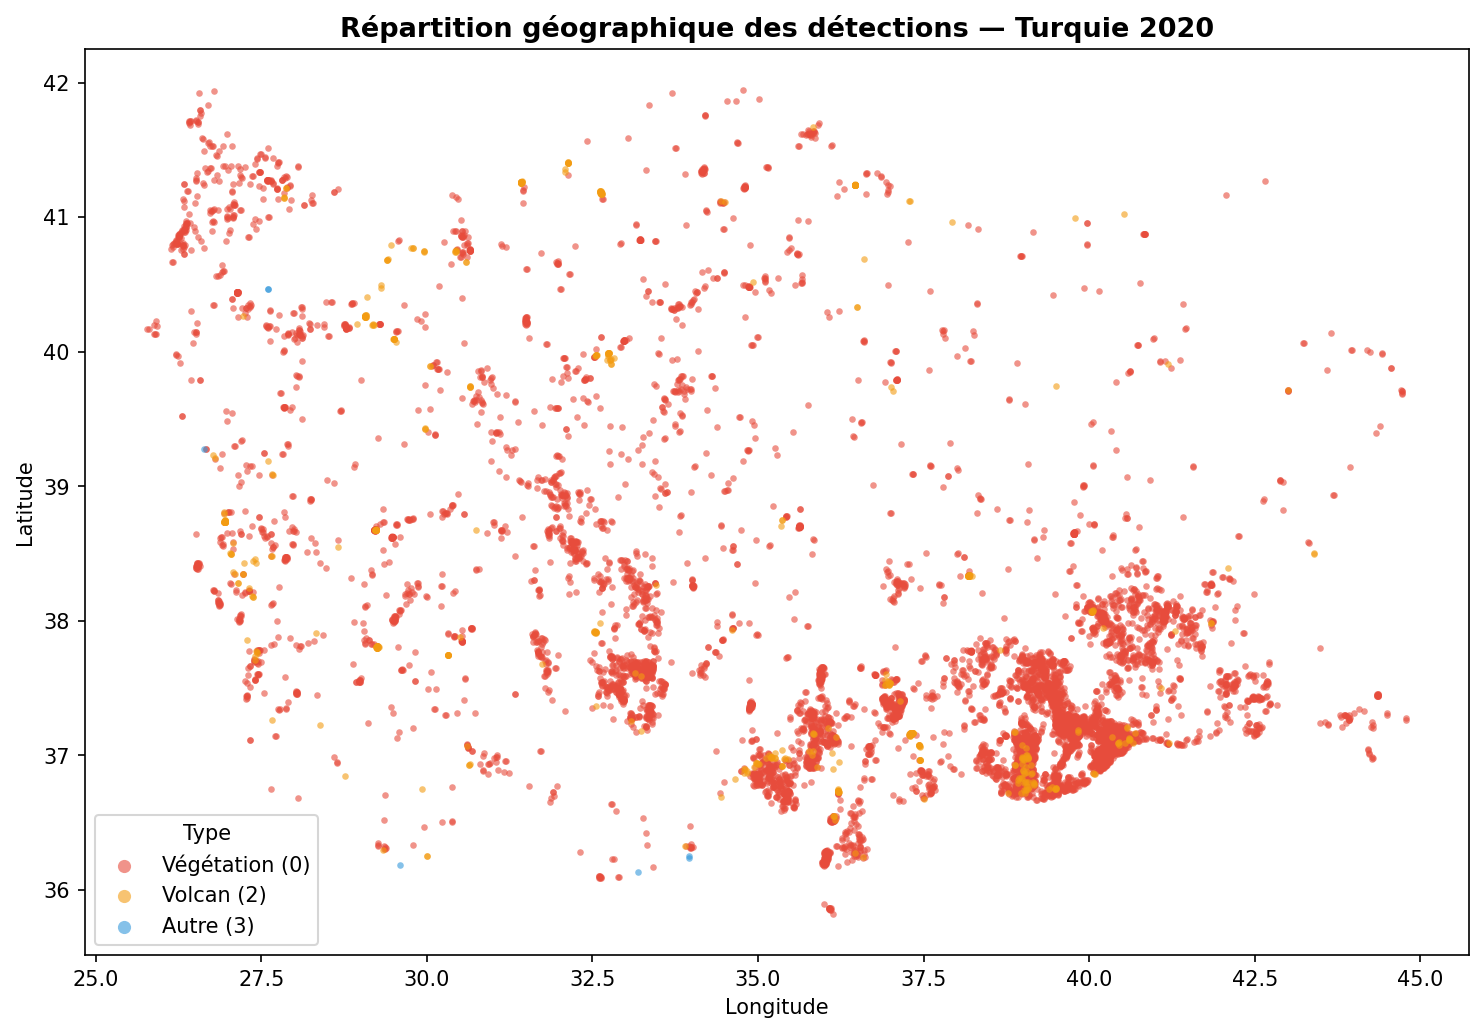
\includegraphics[width=\textwidth]{img/06_carte_geographique.png}
    \caption{Localisation GPS des d\'{e}tections de feux par type -- Turquie 2020}
    \label{fig:carte}
\end{figure}

\section{Conclusion}

L'EDA a mis en \'{e}vidence le fort d\'{e}s\'{e}quilibre des classes, la saisonnalit\'{e} marqu\'{e}e, et les corr\'{e}lations entre features thermiques. Ces observations guident directement le pr\'{e}traitement pr\'{e}sent\'{e} au chapitre suivant.

% ============================================================
% CHAPITRE 3 — PRETRAITEMENT
% ============================================================
\chapter{Pr\'{e}traitement des Donn\'{e}es}

\section{Introduction}

Le pr\'{e}traitement est une \'{e}tape critique : des donn\'{e}es mal pr\'{e}par\'{e}es produisent de mauvais mod\`{e}les m\^{e}me avec les architectures les plus sophistiqu\'{e}es. Ce chapitre d\'{e}crit le pipeline complet de transformation.

\section{Pipeline global}

\begin{table}[H]
\centering
\begin{tabular}{|c|l|l|}
\hline
\rowcolor{bleu!15}
\textbf{\'{E}tape} & \textbf{Action} & \textbf{R\'{e}sultat} \\
\hline
1 & Suppression \texttt{instrument}, \texttt{version} & 15 $\rightarrow$ 13 colonnes \\
\hline
2 & Encodage \texttt{satellite} et \texttt{daynight} & Variables num\'{e}riques 0/1 \\
\hline
3 & Extraction \texttt{mois} et \texttt{heure} depuis les dates & +2 features temporelles \\
\hline
4 & Split strat\'{e}gi\'{e} 80\%/20\% & 7~067 / 1~767 exemples \\
\hline
5A & class\_weight (Pipeline AlexNet) & Poids dans \texttt{model.fit()} \\
\hline
5B & SMOTE (Pipeline ResNet) & 7~067 $\rightarrow$ 19~698 exemples \\
\hline
6 & Normalisation StandardScaler & 12 features normalis\'{e}es \\
\hline
\end{tabular}
\caption{\'{E}tapes du pipeline de pr\'{e}traitement}
\label{tab:pipeline}
\end{table}

\section{Feature Engineering temporel}

La colonne \texttt{acq\_date} est transform\'{e}e en \textbf{mois} (1--12) pour capturer la saisonnalit\'{e}. La colonne \texttt{acq\_time} est convertie en \textbf{heure locale} (0--23). Ces deux features portent une information temporelle directement exploitable.

\section{Gestion du d\'{e}s\'{e}quilibre des classes}

\subsection{Approche 1 --- Class\_weight}

Des poids inversement proportionnels \`{a} la fr\'{e}quence sont calcul\'{e}s :
\begin{equation}
w_i = \frac{N_{\text{total}}}{N_{\text{classes}} \times N_i}
\end{equation}

\begin{table}[H]
\centering
\begin{tabular}{|c|c|p{6cm}|}
\hline
\rowcolor{bleu!15}
\textbf{Classe} & \textbf{Poids} & \textbf{Interpr\'{e}tation} \\
\hline
0 & 0,359 & Peu p\'{e}nalis\'{e}e (majorit\'{e}) \\
\hline
2 & 4,759 & 13$\times$ plus p\'{e}nalis\'{e}e que classe~0 \\
\hline
3 & 392,6 & 1~094$\times$ plus p\'{e}nalis\'{e}e que classe~0 \\
\hline
\end{tabular}
\caption{Poids de classes calcul\'{e}s pour AlexNet-1D}
\label{tab:class_weight}
\end{table}

\subsection{Approche 2 --- SMOTE}

SMOTE g\'{e}n\`{e}re des exemples synth\'{e}tiques par interpolation lin\'{e}aire entre $k$ plus proches voisins :
\begin{equation}
x_{\text{nouveau}} = x_i + \lambda \cdot (x_{\text{voisin}} - x_i), \quad \lambda \sim \mathcal{U}(0,1)
\end{equation}

\begin{figure}[H]
    \centering
    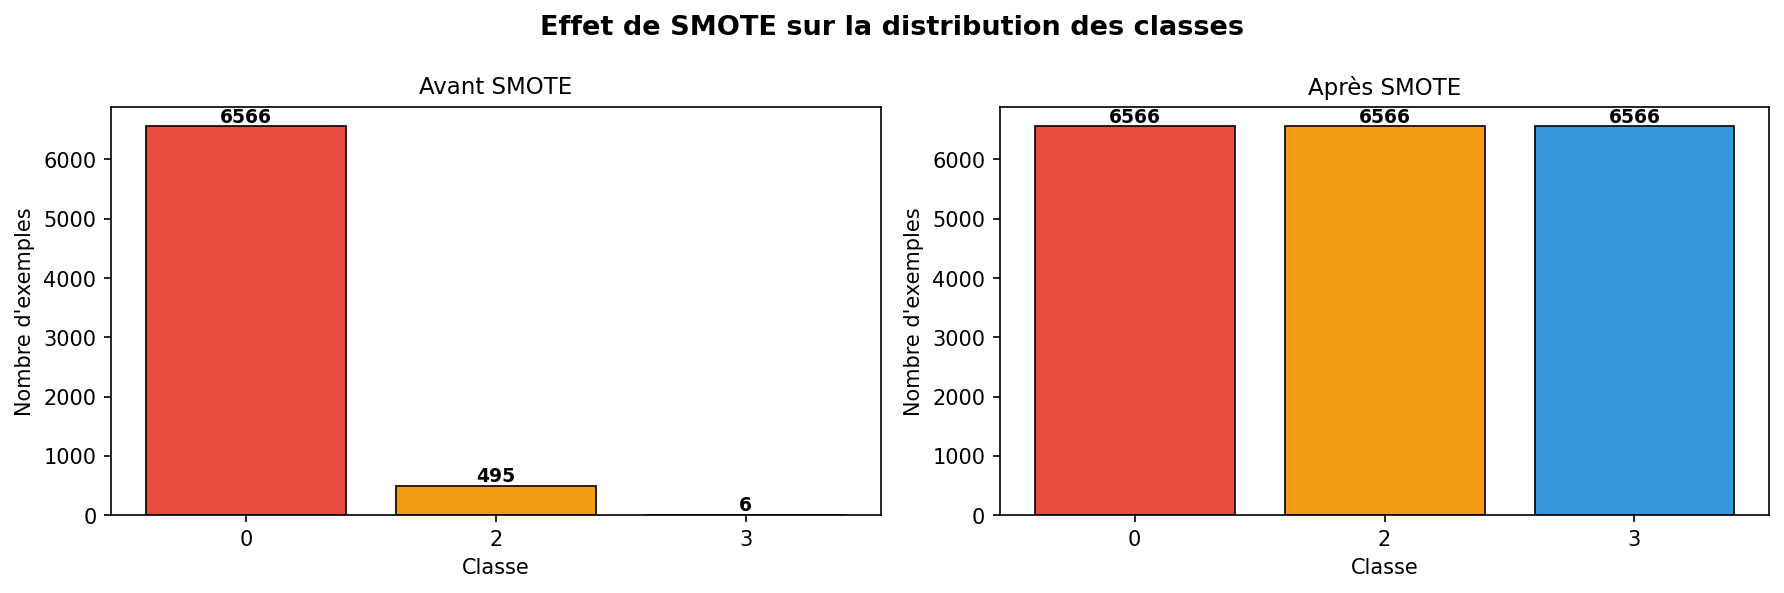
\includegraphics[width=\textwidth]{img/07_smote_comparison.png}
    \caption{Distribution avant/apr\`{e}s SMOTE : 7~067 $\rightarrow$ 19~698 exemples}
    \label{fig:smote}
\end{figure}

\begin{table}[H]
\centering
\begin{tabular}{|c|r|r|r|}
\hline
\rowcolor{bleu!15}
\textbf{Classe} & \textbf{Avant} & \textbf{Apr\`{e}s} & \textbf{Variation} \\
\hline
0 & 6~566 & 6~566 & --- \\
\hline
2 & 495 & 6~566 & +1~226\% \\
\hline
3 & 6 & 6~566 & +109~333\% \\
\hline
\textbf{Total} & \textbf{7~067} & \textbf{19~698} & \textbf{+178\%} \\
\hline
\end{tabular}
\caption{Effet de SMOTE sur le train set}
\label{tab:smote}
\end{table}

\section{Normalisation}

La normalisation z-score est appliqu\'{e}e avec StandardScaler :
\begin{equation}
x' = \frac{x - \mu}{\sigma}
\end{equation}

$\mu$ et $\sigma$ sont calcul\'{e}s uniquement sur le train set et appliqu\'{e}s (transform) sur le test set, \'{e}vitant tout \textit{data leakage}.

\section{Conclusion}

Le pr\'{e}traitement produit 12 features normalis\'{e}es avec deux pipelines parall\`{e}les selon la strat\'{e}gie anti-d\'{e}s\'{e}quilibre. Les donn\'{e}es sont pr\^{e}tes pour les architectures CNN~1D.

% ============================================================
% CHAPITRE 4 — ARCHITECTURES CNN 1D
% ============================================================
\chapter{Architectures CNN 1D pour Donn\'{e}es Tabulaires}

\section{Introduction}

Ce chapitre pr\'{e}sente l'adaptation des CNN aux donn\'{e}es tabulaires et d\'{e}crit les deux mod\`{e}les impl\'{e}ment\'{e}s.

\section{Adaptation tabulaire $\rightarrow$ CNN 1D}

\subsection{Reshape : (n, 12) $\rightarrow$ (n, 12, 1)}

L'API Conv1D de Keras attend \texttt{(batch\_size, steps, channels)}. Chaque feature devient un "pas de temps" avec 1 canal :

\begin{lstlisting}[style=python, caption={Reshape pour Conv1D}]
# Donnees tabulaires (n, 12) --> (n, 12, 1)
X_3d = X.reshape(X.shape[0], 12, 1)
# steps=12 (features), channels=1 (scalaire par feature)
\end{lstlisting}

\subsection{Ordre s\'{e}mantique des features}

Les features sont ordonn\'{e}es par groupe s\'{e}mantique pour maximiser l'information locale captur\'{e}e par les filtres Conv1D :

\begin{center}
\small
[0] latitude \quad [1] longitude \quad [2] brightness \quad [3] scan \quad [4] track\\
[5] satellite \quad [6] confidence \quad [7] bright\_t31 \quad [8] frp \quad [9] daynight \quad [10] mois \quad [11] heure
\end{center}

\section{Architecture 1 --- AlexNet-1D}

Inspir\'{e}e d'AlexNet (Krizhevsky et al., 2012), cette architecture suit une philosophie s\'{e}quentielle : blocs convolutifs enchaîn\'{e}s suivis d'une t\^{e}te de classification dense.

\begin{table}[H]
\centering
\small
\begin{tabular}{|l|c|r|}
\hline
\rowcolor{bleu!15}
\textbf{Couche} & \textbf{Sortie} & \textbf{Param\`{e}tres} \\
\hline
Input & (12, 1) & 0 \\
\hline
Conv1D(64, k=3) + BN + ReLU & (12, 64) & 448 \\
\hline
Conv1D(128, k=3) + BN + ReLU + MaxPool & (6, 128) & 25~088 \\
\hline
Conv1D(256, k=3) + BN + ReLU & (6, 256) & 99~328 \\
\hline
Conv1D(256, k=3) + BN + ReLU & (6, 256) & 197~632 \\
\hline
Conv1D(128, k=3) + BN + ReLU + MaxPool & (3, 128) & 98~816 \\
\hline
GlobalAveragePooling1D & (128,) & 0 \\
\hline
Dense(256) + Dropout(0,5) & (256,) & 33~024 \\
\hline
Dense(128) + Dropout(0,3) & (128,) & 32~896 \\
\hline
\textbf{Dense(3, softmax)} & \textbf{(3,)} & \textbf{387} \\
\hline
\multicolumn{2}{|c|}{\textbf{Total param\`{e}tres}} & \textbf{487~619} \\
\hline
\end{tabular}
\caption{Architecture AlexNet-1D couche par couche}
\label{tab:alexnet_arch}
\end{table}

\section{Architecture 2 --- ResNet-1D}

\subsection{Principe des connexions r\'{e}siduelles}

\begin{equation}
H(x) = F(x) + x \qquad \Rightarrow \qquad
\frac{\partial \mathcal{L}}{\partial x} = \frac{\partial \mathcal{L}}{\partial H} \cdot \left(\frac{\partial F}{\partial x} + 1\right)
\end{equation}

Le terme $+1$ garantit un gradient non nul, \'{e}vitant le \textit{vanishing gradient}.

\begin{lstlisting}[style=python, caption={Bloc r\'{e}siduel ResNet-1D}]
def bloc_residuel(x, n_filtres):
    shortcut = x
    x = Conv1D(n_filtres, 3, padding='same')(x)
    x = BatchNormalization()(x);  x = Activation('relu')(x)
    x = Conv1D(n_filtres, 3, padding='same')(x)
    x = BatchNormalization()(x)
    # Projection si dimensions differentes
    if shortcut.shape[-1] != n_filtres:
        shortcut = Conv1D(n_filtres, 1, padding='same')(shortcut)
        shortcut = BatchNormalization()(shortcut)
    # H(x) = F(x) + x
    x = Add()([x, shortcut])
    return Activation('relu')(x)
\end{lstlisting}

\begin{table}[H]
\centering
\begin{tabular}{|l|c|l|}
\hline
\rowcolor{bleu!15}
\textbf{Stage} & \textbf{Sortie} & \textbf{Composants} \\
\hline
Entr\'{e}e & (12, 64) & Conv1D(64, k=3) + BN + ReLU \\
\hline
Stage 1 & (12, 64) & 2 $\times$ ResBlock(64) \\
\hline
Stage 2 & (12, 128) & 2 $\times$ ResBlock(128) + projection \\
\hline
Stage 3 & (12, 256) & 1 $\times$ ResBlock(256) + projection \\
\hline
T\^{e}te & (3,) & GlobalAvgPool + Dense(128) + Dense(3, softmax) \\
\hline
\multicolumn{2}{|c|}{\textbf{Total param\`{e}tres}} & \textbf{597~443} \\
\hline
\end{tabular}
\caption{Architecture ResNet-1D par stages}
\label{tab:resnet_arch}
\end{table}

\section{Hyperparamètres et callbacks}

\begin{table}[H]
\centering
\begin{tabular}{|l|c|l|}
\hline
\rowcolor{bleu!15}
\textbf{Param\`{e}tre} & \textbf{Valeur} & \textbf{Justification} \\
\hline
Optimiseur & Adam (lr = $10^{-3}$) & Adaptatif, convergence rapide \\
\hline
Fonction de perte & Sparse Categorical CE & Classification multi-classes \\
\hline
Batch size & 32 & Compromis vitesse/stabilit\'{e} \\
\hline
\'{E}poques max & 50 & EarlyStopping arr\^{e}te avant \\
\hline
Validation split & 15\% du train & Suivi de la g\'{e}n\'{e}ralisation \\
\hline
R\'{e}gularisation L2 & $\lambda = 10^{-4}$ & P\'{e}nalise les grands poids \\
\hline
\end{tabular}
\caption{Hyperparam\`{e}tres d'entra\^{i}nement}
\label{tab:hyperparams}
\end{table}

\section{Conclusion}

Les deux architectures CNN~1D constituent des adaptations fid\`{e}les d'AlexNet et ResNet aux donn\'{e}es tabulaires. Leurs performances sont \'{e}valu\'{e}es au chapitre suivant.

% ============================================================
% CHAPITRE 5 — RESULTATS
% ============================================================
\chapter{R\'{e}sultats et \'{E}valuation}

\section{Introduction}

Ce chapitre pr\'{e}sente les m\'{e}triques d'\'{e}valuation, les r\'{e}sultats obtenus et la comparaison des deux architectures.

\section{M\'{e}triques d'\'{e}valuation}

\begin{table}[H]
\centering
\begin{tabular}{|l|p{4.5cm}|p{5cm}|}
\hline
\rowcolor{bleu!15}
\textbf{M\'{e}trique} & \textbf{Formule} & \textbf{Pertinence} \\
\hline
Accuracy & $\frac{TP + TN}{N}$ & R\'{e}f\'{e}rence globale (insuffisante seule) \\
\hline
Precision & $\frac{TP}{TP + FP}$ (weighted) & Taux de vrais positifs \\
\hline
Recall & $\frac{TP}{TP + FN}$ (weighted) & Taux de d\'{e}tection \\
\hline
\textbf{F1-score} & $\frac{2 \times P \times R}{P + R}$ & \textbf{M\'{e}trique principale} \\
\hline
RMSE & $\sqrt{\frac{1}{N}\sum(y-\hat{y})^2}$ & Amplitude des erreurs \\
\hline
\end{tabular}
\caption{M\'{e}triques d'\'{e}valuation utilis\'{e}es}
\label{tab:metriques}
\end{table}

\section{Courbes d'entra\^{i}nement}

\begin{figure}[H]
    \centering
    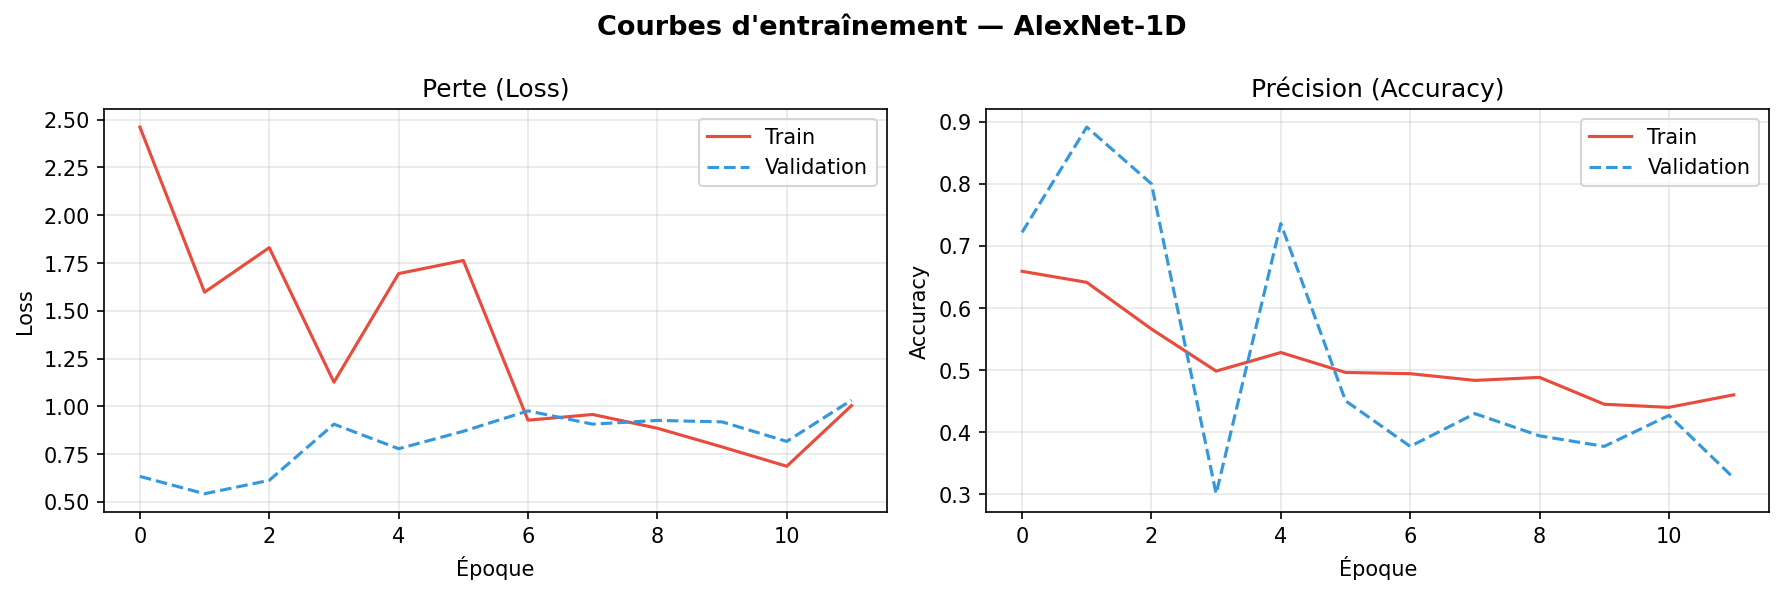
\includegraphics[width=\textwidth]{img/08_courbes_alexnet_1d.png}
    \caption{Courbes AlexNet-1D : meilleure \'{e}poque = 2, EarlyStopping \`{a} l'\'{e}poque 12}
    \label{fig:courbes_alex}
\end{figure}

\begin{figure}[H]
    \centering
    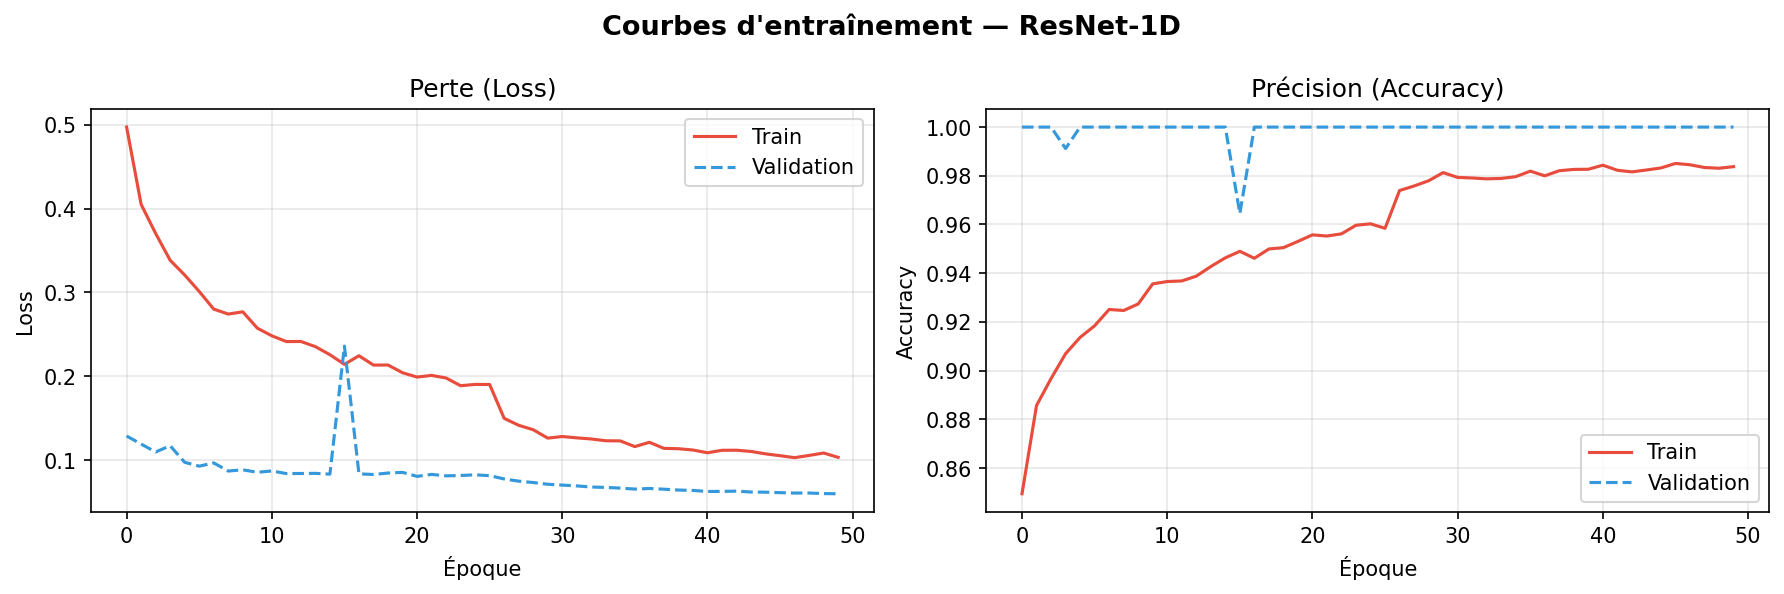
\includegraphics[width=\textwidth]{img/08_courbes_resnet_1d.png}
    \caption{Courbes ResNet-1D : 50 \'{e}poques compl\`{e}tes, val\_accuracy = 100\%, val\_loss = 0,0602}
    \label{fig:courbes_res}
\end{figure}

\section{Matrices de confusion}

\begin{figure}[H]
    \centering
    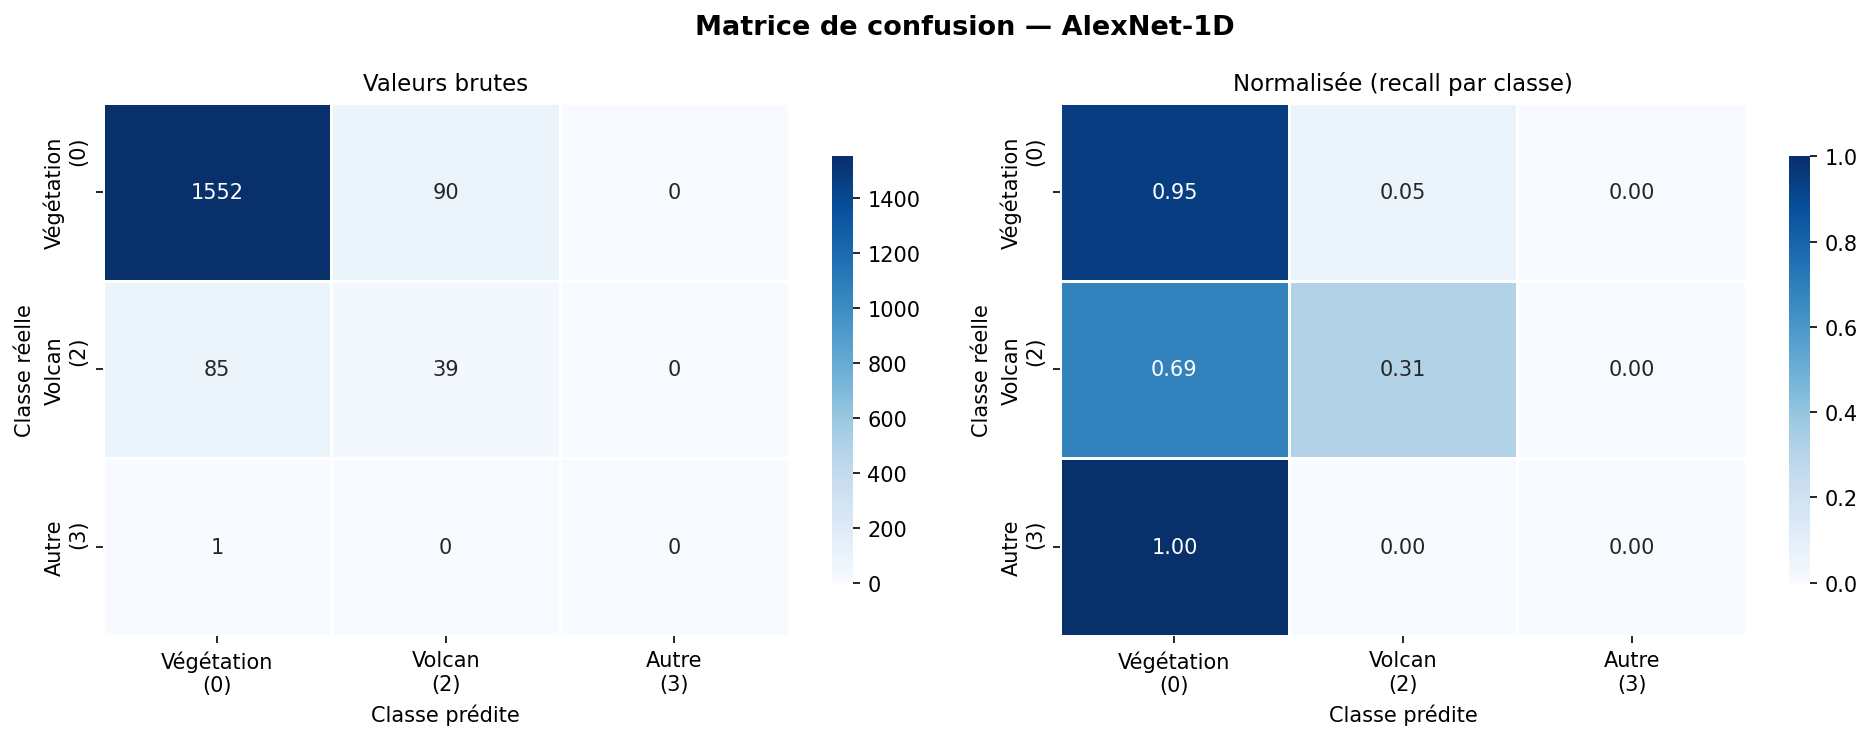
\includegraphics[width=\textwidth]{img/09_confusion_alexnet_1d.png}
    \caption{Matrices de confusion AlexNet-1D (brute et normalis\'{e}e)}
    \label{fig:cm_alex}
\end{figure}

\begin{figure}[H]
    \centering
    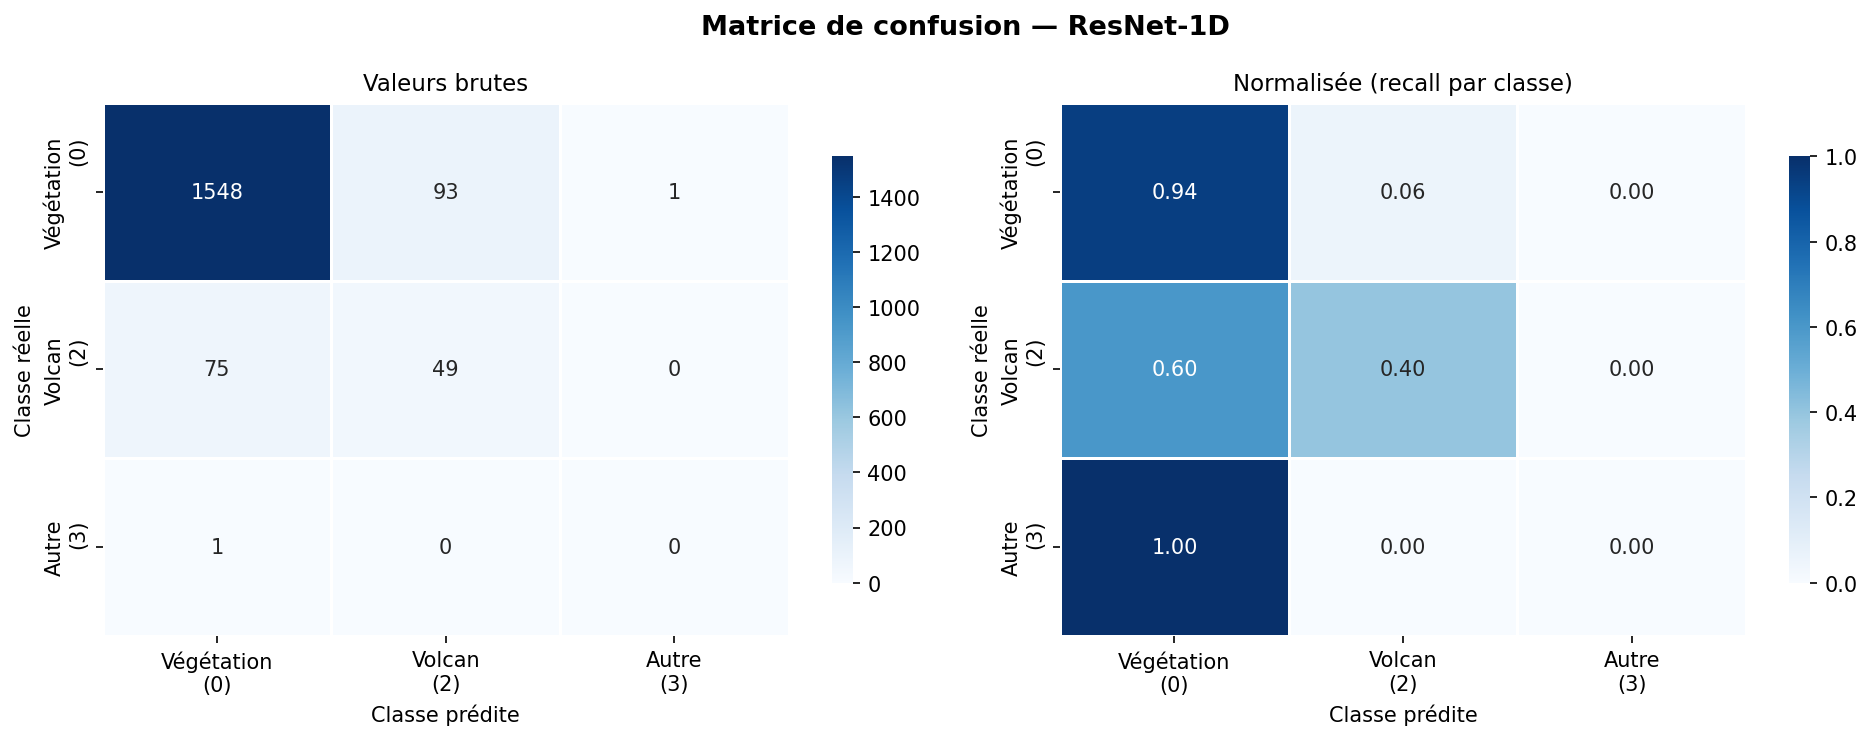
\includegraphics[width=\textwidth]{img/09_confusion_resnet_1d.png}
    \caption{Matrices de confusion ResNet-1D (brute et normalis\'{e}e)}
    \label{fig:cm_res}
\end{figure}

\section{Rapport de classification par classe}

\begin{table}[H]
\centering
\begin{tabular}{|l|c|c|c|c|}
\hline
\rowcolor{bleu!15}
\multicolumn{5}{|c|}{\textbf{AlexNet-1D (class\_weight) --- Meilleure \'{e}poque : 2}} \\
\hline
\textbf{Classe} & \textbf{Pr\'{e}cision} & \textbf{Rappel} & \textbf{F1} & \textbf{Support} \\
\hline
0 --- V\'{e}g\'{e}tation & 0,95 & 0,95 & 0,95 & 1~642 \\
\hline
2 --- Volcan & 0,30 & 0,31 & 0,31 & 124 \\
\hline
3 --- Autre & 0,00 & 0,00 & 0,00 & 1 \\
\hline
\rowcolor{grislight}
\textbf{Weighted avg} & \textbf{0,90} & \textbf{0,90} & \textbf{0,90} & \textbf{1~767} \\
\hline
\end{tabular}
\caption{Rapport de classification AlexNet-1D}
\label{tab:report_alex}
\end{table}

\begin{table}[H]
\centering
\begin{tabular}{|l|c|c|c|c|}
\hline
\rowcolor{vert!15}
\multicolumn{5}{|c|}{\textbf{ResNet-1D (SMOTE) --- 50 \'{e}poques}} \\
\hline
\textbf{Classe} & \textbf{Pr\'{e}cision} & \textbf{Rappel} & \textbf{F1} & \textbf{Support} \\
\hline
0 --- V\'{e}g\'{e}tation & 0,95 & 0,94 & 0,95 & 1~642 \\
\hline
2 --- Volcan & 0,35 & 0,40 & 0,37 & 124 \\
\hline
3 --- Autre & 0,00 & 0,00 & 0,00 & 1 \\
\hline
\rowcolor{grislight}
\textbf{Weighted avg} & \textbf{0,91} & \textbf{0,90} & \textbf{0,91} & \textbf{1~767} \\
\hline
\end{tabular}
\caption{Rapport de classification ResNet-1D}
\label{tab:report_res}
\end{table}

\section{Tableau comparatif final}

\begin{table}[H]
\centering
\begin{tabular}{|l|c|c|c|c|c|c|}
\hline
\rowcolor{bleu!15}
\textbf{Mod\`{e}le} & \textbf{Strat\'{e}gie} & \textbf{Accuracy} & \textbf{Precision} & \textbf{Recall} & \textbf{F1} & \textbf{RMSE} \\
\hline
AlexNet-1D & class\_weight & 90,04\% & 90,17\% & 90,04\% & 90,10\% & 0,6334 \\
\hline
\rowcolor{vert!10}
\textbf{ResNet-1D} & \textbf{SMOTE} & \textbf{90,38\%} & \textbf{91,00\%} & \textbf{90,38\%} & \textbf{90,67\%} & \textbf{0,6249} \\
\hline
\end{tabular}
\caption{Comparaison finale des deux architectures CNN 1D}
\label{tab:comparaison}
\end{table}

\begin{figure}[H]
    \centering
    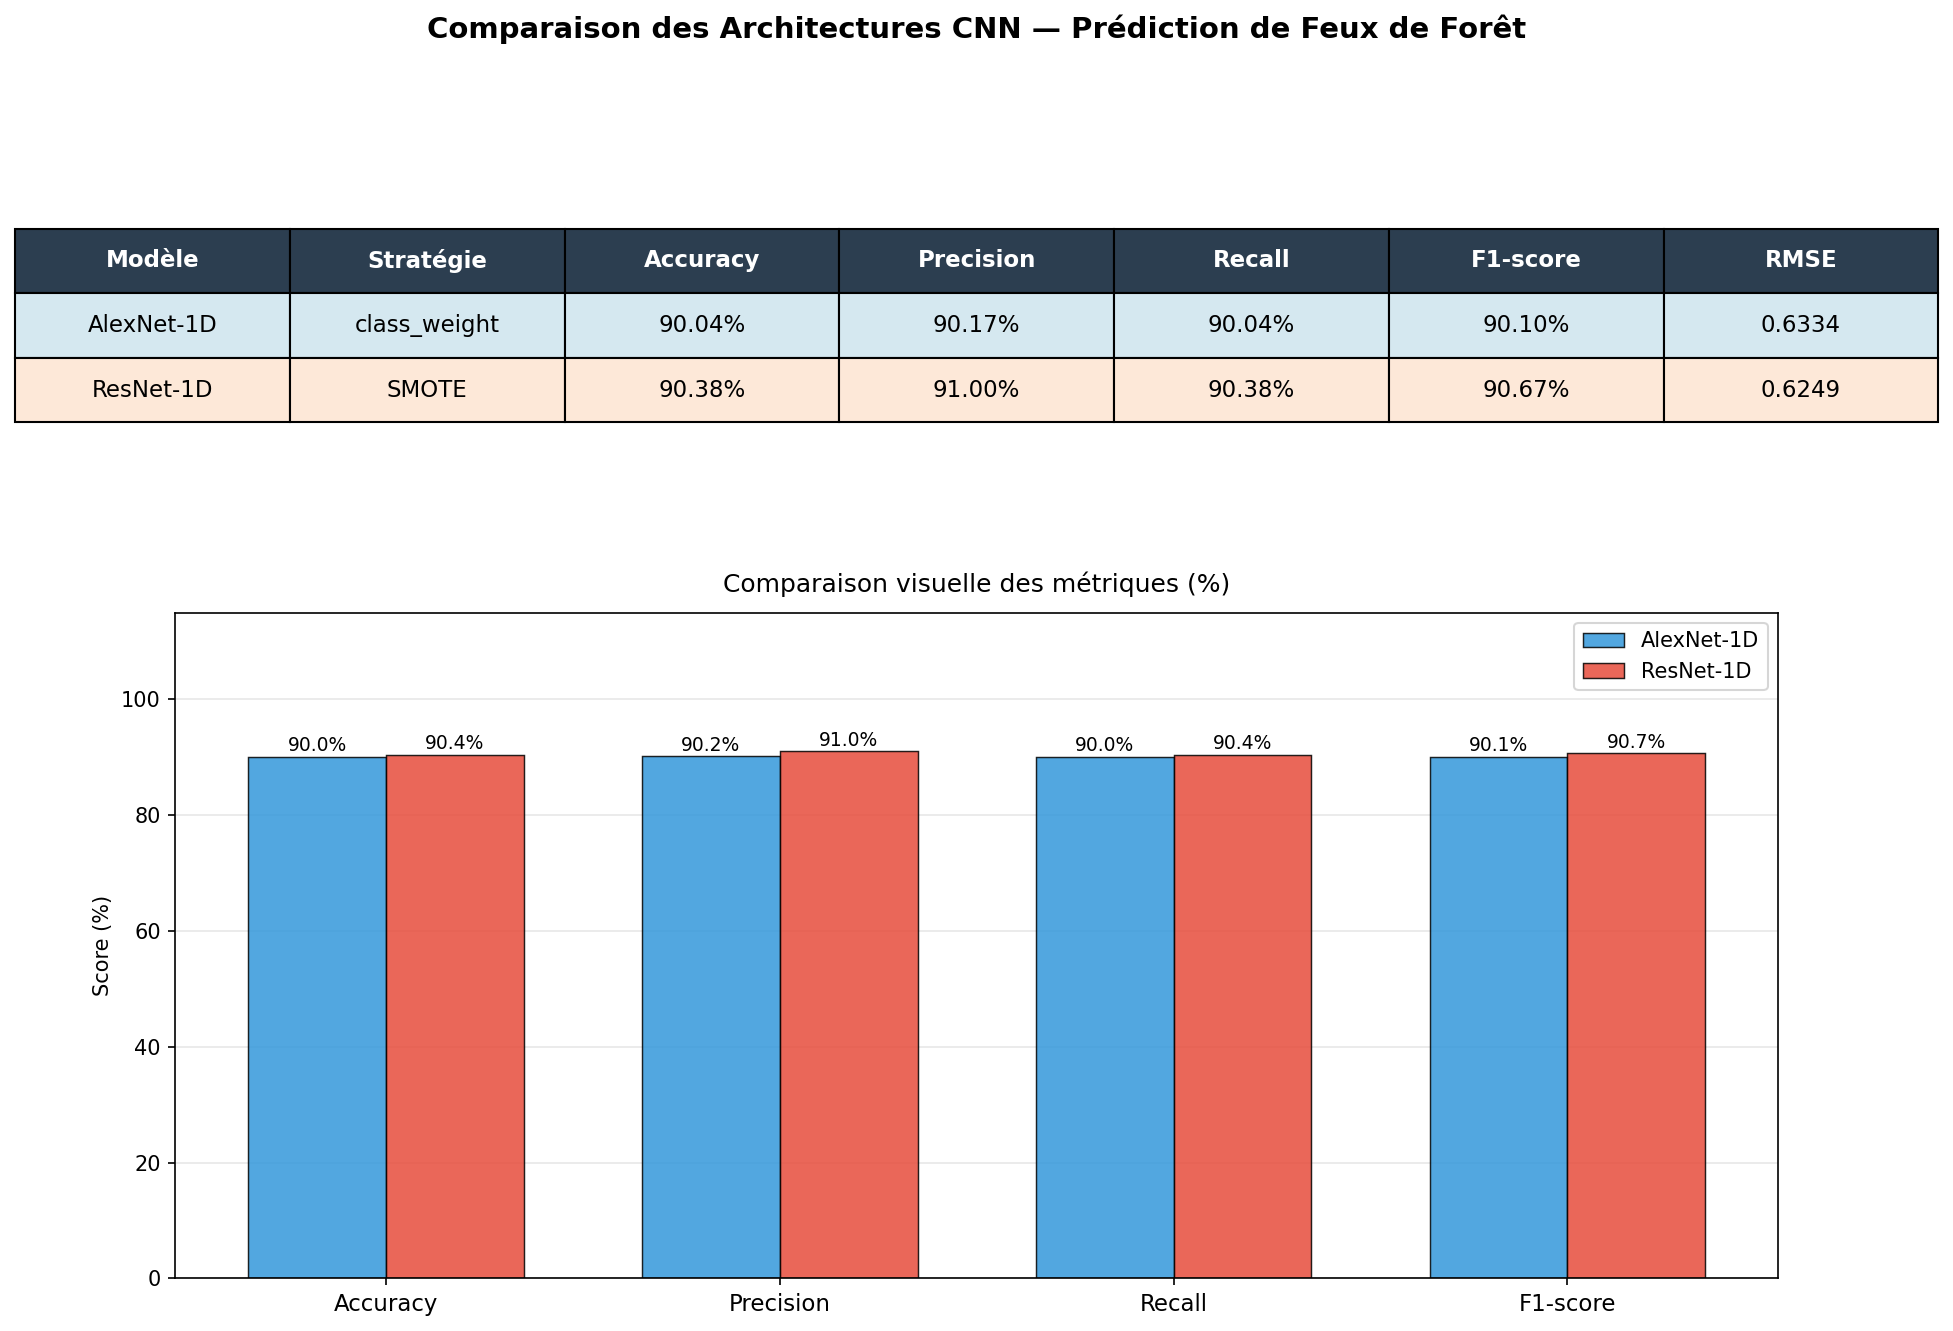
\includegraphics[width=\textwidth]{img/10_comparaison_finale.png}
    \caption{Visualisation comparative --- ResNet-1D domine sur tous les indicateurs}
    \label{fig:comparaison}
\end{figure}

\section{Discussion}

\subsection{Analyse}

\begin{itemize}
    \item \textbf{ResNet-1D} surpasse AlexNet-1D sur toutes les m\'{e}triques. Le gain le plus notable concerne le recall de la classe~2 (volcans) : \textbf{40\%} vs \textbf{31\%}, soit +29\% relatif
    \item SMOTE a fourni davantage d'exemples synth\'{e}tiques de volcans, am\'{e}liorant l'apprentissage de leurs caract\'{e}ristiques
    \item Les connexions r\'{e}siduelles ont permis une convergence plus stable sur 50 \'{e}poques
\end{itemize}

\subsection{Limites}

\begin{enumerate}
    \item \textbf{Classe~3 ind\'{e}tectable} : 7 exemples au total (1 en test) --- F1 = 0,00
    \item \textbf{SMOTE sur donn\'{e}es mixtes} : features binaires g\'{e}n\`{e}rent des valeurs interpol\'{e}es non r\'{e}alistes
    \item \textbf{S\'{e}quence courte} : 12 features limitent la profondeur effective des filtres
\end{enumerate}

\section{Conclusion}

ResNet-1D avec SMOTE est la meilleure configuration : F1 = 90,67\% et RMSE = 0,6249. Ces r\'{e}sultats sont exploit\'{e}s dans l'application web pr\'{e}sent\'{e}e au chapitre suivant.

% ============================================================
% CHAPITRE 6 — APPLICATION WEB
% ============================================================
\chapter{Application Web --- FireRisk AI}

\section{Introduction}

Ce chapitre pr\'{e}sente \textbf{FireRisk AI}, application web d\'{e}velopp\'{e}e avec Streamlit, permettant de pr\'{e}dire le risque d'incendie en temps r\'{e}el.

\section{Technologies utilis\'{e}es}

\begin{table}[H]
\centering
\begin{tabular}{|c|c|p{6cm}|}
\hline
\rowcolor{bleu!15}
\textbf{Technologie} & \textbf{Version} & \textbf{R\^{o}le} \\
\hline
Python & 3.11+ & Langage principal \\
\hline
Streamlit & 1.x & Framework web interactif \\
\hline
TensorFlow / Keras & 2.x & Chargement et inf\'{e}rence du mod\`{e}le \\
\hline
Folium & 0.14+ & Carte interactive (Leaflet.js) \\
\hline
streamlit-folium & 0.x & Int\'{e}gration Folium $\leftrightarrow$ Streamlit \\
\hline
scikit-learn & 1.2+ & StandardScaler (normalisation) \\
\hline
joblib & 1.2+ & S\'{e}rialisation du scaler \\
\hline
\end{tabular}
\caption{Stack technologique de l'application FireRisk AI}
\label{tab:stack}
\end{table}

\section{Fonctionnalit\'{e}s principales}

\subsection{Deux modes de saisie synchronis\'{e}s}

L'utilisateur peut d\'{e}finir la localisation de deux fa\c{c}ons :

\begin{enumerate}
    \item \textbf{Clic sur la carte interactive} : un clic sur la carte Folium d\'{e}place le marqueur et met \`{a} jour les coordonn\'{e}es via \texttt{st.session\_state}
    \item \textbf{Saisie manuelle} : champs \texttt{number\_input} dans le panneau lat\'{e}ral avec bornes mondiales ($-90°$ \`{a} $90°$ en latitude, $-180°$ \`{a} $180°$ en longitude)
\end{enumerate}

Un badge vert/orange indique si la position est dans la zone d'entra\^{i}nement (Turquie).

\subsection{Niveaux de risque}

\begin{table}[H]
\centering
\begin{tabular}{|c|p{6cm}|c|}
\hline
\rowcolor{bleu!15}
\textbf{Niveau} & \textbf{Conditions} & \textbf{Couleur} \\
\hline
\textbf{CRITIQUE} & Type v\'{e}g\'{e}tation + $p_{\text{v\'{e}g}} > 0,75$ + FRP $> 100$ MW & Rouge \\
\hline
\textbf{\'{E}LEV\'{E}} & Type v\'{e}g\'{e}tation + $p_{\text{v\'{e}g}} > 0,55$ + FRP $> 30$ MW & Orange \\
\hline
\textbf{MOD\'{E}R\'{E}} & Type v\'{e}g\'{e}tation (faible intensit\'{e}) ou volcan & Jaune \\
\hline
\textbf{FAIBLE} & Type autre source & Vert \\
\hline
\textbf{AUCUN} & brightness $< 305$~K + FRP $< 3$ MW + confiance $< 25\%$ & Bleu \\
\hline
\end{tabular}
\caption{Niveaux de risque et conditions de d\'{e}clenchement}
\label{tab:risk}
\end{table}

\subsection{Historique des analyses}

Chaque analyse est automatiquement enregistr\'{e}e dans \texttt{st.session\_state}. L'historique (20 derni\`{e}res analyses) est affich\'{e} en bas de page avec :
\begin{itemize}
    \item Horodatage, niveau de risque, type d\'{e}tect\'{e}
    \item Coordonn\'{e}es GPS, FRP, brightness, confiance MODIS
    \item Probabilit\'{e}s des 3 classes
    \item Export CSV t\'{e}l\'{e}chargeable
\end{itemize}

\section{Correction du bug de persistance}

\begin{infobox}
\textbf{Probl\`{e}me :} Streamlit r\'{e}ex\'{e}cute le script entier \`{a} chaque interaction (rendu de carte, d\'{e}placement de slider). Sans \texttt{session\_state}, les r\'{e}sultats disparaissaient d\`{e}s que la carte Folium se chargeait.

\textbf{Solution :} Les r\'{e}sultats sont stock\'{e}s dans \texttt{st.session\_state["last\_result"]} d\`{e}s qu'une pr\'{e}diction est effectu\'{e}e, et affich\'{e}s depuis cette m\'{e}moire persistante \`{a} chaque rerun.
\end{infobox}

\section{Pipeline de pr\'{e}diction}

\begin{lstlisting}[style=python, caption={Pipeline complet de pr\'{e}diction dans l'application}]
def predire(latitude, longitude, brightness, ...):
    # 1. Encodage categoriel
    sat_enc = 0 if satellite == "Terra (A)" else 1
    dn_enc  = 0 if daynight  == "Jour (D)"  else 1
    # 2. Construction du vecteur de features
    X = np.array([[latitude, longitude, brightness, scan, track,
                   sat_enc, confidence, bright_t31, frp,
                   dn_enc, mois, heure]], dtype=float)
    # 3. Normalisation
    X_scaled = scaler.transform(X)
    # 4. Reshape pour Conv1D : (1, 12) --> (1, 12, 1)
    X_3d = X_scaled.reshape(1, 12, 1)
    # 5. Prediction ResNet-1D
    probas = model.predict(X_3d, verbose=0)[0]
    # 6. Remap labels : {0,1,2} --> {0,2,3}
    inv_map = {0: 0, 1: 2, 2: 3}
    type_reel = inv_map[int(np.argmax(probas))]
    # 7. Calcul du niveau de risque
    return calculer_risque(type_reel, probas[0], frp, confidence)
\end{lstlisting}

\section{Lancement}

\begin{lstlisting}[style=python, caption={Commande de lancement}]
streamlit run app.py
# Accessible sur : http://localhost:8501
\end{lstlisting}

\section{Conclusion}

FireRisk AI offre une interface intuitive permettant \`{a} tout utilisateur d'\'{e}valuer le risque d'incendie en temps r\'{e}el, avec s\'{e}lection de localisation par carte interactive et historique complet des analyses.

% ============================================================
% CONCLUSION GENERALE
% ============================================================
\chapter*{Conclusion g\'{e}n\'{e}rale}
\addcontentsline{toc}{chapter}{Conclusion g\'{e}n\'{e}rale}

\justifying
Ce projet de fin d'ann\'{e}es a permis de concevoir et valider un \textbf{pipeline complet de classification des feux de for\^{e}t} \`{a} partir de donn\'{e}es satellitaires MODIS, en s'appuyant sur des architectures CNN~1D adapt\'{e}es aux donn\'{e}es tabulaires.

\medskip
\textbf{Bilan des contributions :}
\begin{itemize}
    \item \textbf{EDA} : mise en \'{e}vidence du fort d\'{e}s\'{e}quilibre (1172:1), de la saisonnalit\'{e} estivale et de l'importance du FRP comme feature discriminante
    \item \textbf{Pr\'{e}traitement} : pipeline robuste avec deux strat\'{e}gies anti-d\'{e}s\'{e}quilibre (class\_weight vs SMOTE)
    \item \textbf{Mod\'{e}lisation} : deux architectures CNN~1D impl\'{e}ment\'{e}es et compar\'{e}es
    \item \textbf{R\'{e}sultats} : ResNet-1D + SMOTE atteint \textbf{F1 = 90,67\%} et RMSE = 0,6249
    \item \textbf{Application} : FireRisk AI avec pr\'{e}diction en temps r\'{e}el et s\'{e}lection par carte interactive
\end{itemize}

\medskip
\textbf{Perspectives :}
\begin{itemize}
    \item SMOTE-NC pour les features cat\'{e}gorielles mixtes
    \item Collecte de donn\'{e}es pour la classe~3 (7 exemples insuffisants)
    \item TabTransformer pour une meilleure repr\'{e}sentation tabulaire
    \item Extension g\'{e}ographique \`{a} d'autres pays m\'{e}diterran\'{e}ens
    \item Connexion temps r\'{e}el \`{a} l'API NASA FIRMS
\end{itemize}

% ============================================================
% BIBLIOGRAPHIE
% ============================================================
\chapter*{Bibliographie}
\addcontentsline{toc}{chapter}{Bibliographie}

\begin{enumerate}[leftmargin=1.5cm, label={[\arabic*]}]

    \item Krizhevsky, A., Sutskever, I., \& Hinton, G. E. (2012). \textit{ImageNet classification with deep convolutional neural networks}. Advances in Neural Information Processing Systems, 25, 1097--1105.

    \item He, K., Zhang, X., Ren, S., \& Sun, J. (2016). \textit{Deep residual learning for image recognition}. Proceedings of the IEEE CVPR, 770--778.

    \item Chawla, N. V., Bowyer, K. W., Hall, L. O., \& Kegelmeyer, W. P. (2002). \textit{SMOTE: Synthetic minority over-sampling technique}. Journal of Artificial Intelligence Research, 16, 321--357.

    \item Giglio, L., Schroeder, W., \& Justice, C. O. (2016). \textit{The collection 6 MODIS active fire detection algorithm and fire products}. Remote Sensing of Environment, 178, 31--41.

    \item Kiranyaz, S., et al. (2021). \textit{1D convolutional neural networks and applications: A survey}. Mechanical Systems and Signal Processing, 151, 107398.

    \item He, H., \& Garcia, E. A. (2009). \textit{Learning from imbalanced data}. IEEE Transactions on Knowledge and Data Engineering, 21(9), 1263--1284.

    \item Simonyan, K., \& Zisserman, A. (2014). \textit{Very deep convolutional networks for large-scale image recognition}. arXiv:1409.1556.

    \item Hochreiter, S., \& Schmidhuber, J. (1997). \textit{Long short-term memory}. Neural Computation, 9(8), 1735--1780.

    \item Chollet, F. (2021). \textit{Deep Learning with Python} (2nd ed.). Manning Publications.

    \item Pedregosa, F., et al. (2011). \textit{Scikit-learn: Machine learning in Python}. Journal of Machine Learning Research, 12, 2825--2830.

    \item NASA FIRMS. (2020). \textit{Fire Information for Resource Management System}. \url{https://earthdata.nasa.gov/firms}

    \item LeCun, Y., et al. (1998). \textit{Gradient-based learning applied to document recognition}. Proceedings of the IEEE, 86(11), 2278--2324.

\end{enumerate}

\end{document}
